%%%%%%%%%%%%%%%%%%%%%%%%%%%%%%%%%%%%%%%%%%%%%%%%%%%%%%%%%%%%%%%%%%%%%%%%%%%%%%%%
%2345678901234567890123456789012345678901234567890123456789012345678901234567890
%        1         2         3         4         5         6         7         8

\documentclass[letterpaper, 10 pt, conference]{ieeeconf}  % Comment this line out if you need a4paper
%\documentclass[a4paper, 10pt, conference]{ieeeconf}      % Use this line for a4 paper

\IEEEoverridecommandlockouts                              % This command is only needed if you want to use the \thanks command
\overrideIEEEmargins                                      % Needed to meet printer requirements.

% --- Graphics and fonts
\usepackage{graphicx}
\graphicspath{{figures/}}
\usepackage{epsfig}
\usepackage{mathptmx}
\usepackage{times}

% --- Math
\usepackage{amsmath}
\usepackage{amssymb}

% --- Tables / alignment helpers
\usepackage{array}

% --- Units, angles, URLs and links
\usepackage{siunitx}
\sisetup{per-mode=symbol} % 110 r/min style
% Use plain text for "r" and exponent for min^{-1}; avoids nested \per
\DeclareSIUnit{\rpm}{\text{r\,min^{-1}}}

\sisetup{
  reset-text-series = false,
  text-series-to-math = true,
  reset-text-family = false,
  text-family-to-math = true,
  per-mode = symbol,
  group-minimum-digits = 4
}
\usepackage[hyphens]{url}
\usepackage[hidelinks]{hyperref}
\urlstyle{same}
\Urlmuskip=0mu plus 1mu\relax
\def\UrlBreaks{\do\/\do-\do\.\do\_}

\title{\LARGE \bf
LEAPONE: Design of a Six-Wheeled Rover with Integrated Sampling Systems for Remote Mars Analogue Missions
}

\author{Ayan Akbar Ali$^{1}$, Brahama Teja Naroju$^{1}$, Danny Sneham$^{1}$, Harsha Vardhan Raju Gottimukkala$^{1}$, Kiran Achari$^{2}$,\\ Swaraj Tendulkar$^{1}$, Frank Schrödel$^{1}$ % <-this % stops a space
\thanks{*We gratefully acknowledge the financial support for this research by the Thüringer Ministeriums für Bildung, Wissenschaft und Kultur for the project Hochschulübergreifende Forschungsgruppe Vernetztes und Kognitives Fahren.}% <-this % stops a space
\thanks{Ayan Akbar Ali$^{1}$, Brahama Teja Naroju$^{1}$, Danny Sneham$^{1}$, Harsha Vardhan Raju Gottimukkala$^{1}$, Swaraj Tendulkar$^{1}$ and Frank Schrödel$^{1}$ are with the Faculty of Mechanical Engineering, Schmalkalden University of Applied Sciences, 98574 Schmalkalden, Germany.}
\thanks{Kiran Achari$^{2}$ is with Boehm System Engineering GmbH, Germany.}
}

\begin{document}

\maketitle
\thispagestyle{empty}
\pagestyle{empty}

%%%%%%%%%%%%%%%%%%%%%%%%%%%%%%%%%%%%%%%%%%%%%%%%%%%%%%%%%%%%%%%%%%%%%%%%%%%%%%%%
\begin{abstract}
This paper presents the LEAPONE rover platform inspired from the existing planetary exploration solutions developed specifically for remote Mars analogue missions. The paper introduces the mechanical design of the 6-wheeled rover base powered by a rocker bogie suspension for terrain navigation equipped with a custom designed robotic arm for sampling and a telescopic drill for subsurface exploration. The LEAPONE rover is designed to compete in the European Rover Challenge (ERC) organized in Poland through the European Space Foundation. The competition presents a variety of tasks similar to the ones performed on the Mars on a constructed Mars yard. Out of the different tasks, the main tasks considered in this paper are Navigation, Surface Sampling and Deep Sampling. In addition to the mechanical design, the paper details the electrical system and communication architecture that enable remote operation throughout the mission time frame. These developments highlight an integrated approach to designing versatile planetary rovers for both research and competition scenarios. 
\end{abstract}

%%%%%%%%%%%%%%%%%%%%%%%%%%%%%%%%%%%%%%%%%%%%%%%%%%%%%%%%%%%%%%%%%%%%%%%%%%%%%%%%
\section{INTRODUCTION}
Space robotics can be considered a niche field of engineering in which the conditions given by the space environment present particular constraints to the research activities conducted in the area. The space environment is harsh and remote and difficult to access. Restrictions with respect to the available technology and components for space can sometimes be years behind their terrestrial counterparts and more drastically in the system mass and energy. This leads to the need for highly optimized and customized systems. \cite{marstestbed} The Mars Exploration Rovers represent a great advance in planetary rover technology since their predecessor, the rover ‘Sojourner’, explored the local vicinity around the Mars Pathfinder lander in 1997 \cite{mobsub}. Autonomous robots for exploration of extraterrestrial surfaces require reliable and robust locomotion systems \cite{sherpasus}. To test autonomous robotic solutions for space exploration and tasks from around the world, the European Rover Challenge (ERC) is held each year in which teams perform tasks analogous to those of rovers on the surface of Mars \cite{ERC20}. The competition aims at stimulating and supporting a new generation of engineers by developing competencies, skills, and networks within the space sector \cite{ERC20}. This paper introduces a space robotic platform compliant with the ERC guidelines developed by HSM Aries \cite{aries} at Hochschule Schmalkalden.   

\section{STATE OF THE ART}
For Mars exploration, rocker bogie mechanisms are successfully deployed on Mars rovers so far \cite{b1}, \cite{b2}, \cite{b3}. The passive suspension systems like the rocker bogie mechanisms help in overcoming obstacles in the size of the order of the wheel diameters \cite{sherpasus}. The rovers Spirit and Opportunity developed by NASA were 6-wheel drive, 4-wheel steered vehicles with a rocker bogie suspension system similar in design to their predecessor, Sojourner, the rover sent to Mars on the Mars Pathfinder mission in 1996 \cite{b1}, \cite{b4}. In Fig. \ref{spirit-sherpa} the Spirit rover is shown performing its first drive in the Spacecraft Assembly Facility at JPL \cite{b1}. The SherpaTT rover developed by the DFKI Robotics Innovation Center, Bremen illustrated in Fig. \ref{spirit-sherpa} employs a hybrid-leg system featuring an active articulated suspension system comprising four legs with actively driven and steered wheels at each leg's end \cite{sherpasus}.  
    \begin{figure}[htbp]
    \centerline{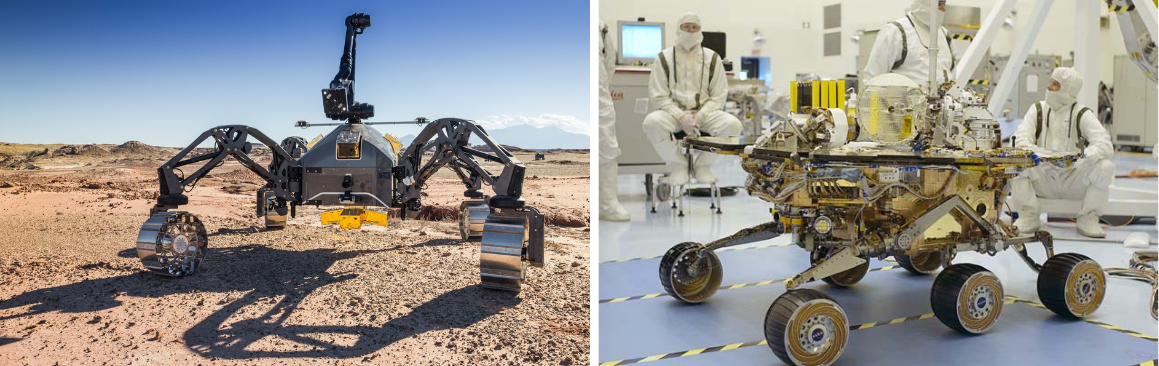
\includegraphics[width=85mm]{Sprirt-sherpa.png}}
    \caption{The SherpaTT rover [Left Image] and Flight Rover ‘Spirit’ in the JPL Spacecraft Assembly Facility [Right Image] \cite{sherpasus}, \cite{b2}}
    \label{spirit-sherpa}
    \end{figure}

The newest version of the NASA rovers, was the Perseverance rover on a science driven mission requiring it to drive long distances and collecting diverse set of samples at distinct geological regions. In the first two years, Perseverance drove 17.7 km and drilled sample cores sealing 23 sample tubes and depositing 10 of those at a location on Mars for potential pickup by the Mars Sample Retrieval Helicopters. \cite{b5} Furthermore, under the leadership of H. Das of JPL, \cite{b6} illustrated the autonomous acquisition of small rocks, using visual and touch sensors and a rover-mounted micro-arm to achieve the rock pick-up operation. The Rocky 7 rover \cite{b7} was used as the platform for this demonstration. This paper takes inspiration from the state of the art and introduces the robotic platform LEAP-ONE. The rover is constructed to participate in the European Rover Challenge and perform the tasks put forth by the competition organizers. The next section provides an overview of the tasks in the competition for which the rover is designed. 

\section{PROBLEM STATEMENT}
The European Rover Challenge (ERC) aims to advance and test technological competence with an emphasis on applications in space exploration. Its principal objective is to offer a standardized testing ground for constructing robotic systems capable of executing mission-oriented tasks within a simulated extraterrestrial Mars environment. These tasks are aligned with internationally recognized roadmaps for space robotics, thereby reflecting the complexity and challenges anticipated in future industry applications. This paper focuses on three of the main tasks assigned by the ERC.
    \begin{figure}[htbp]
    \centerline{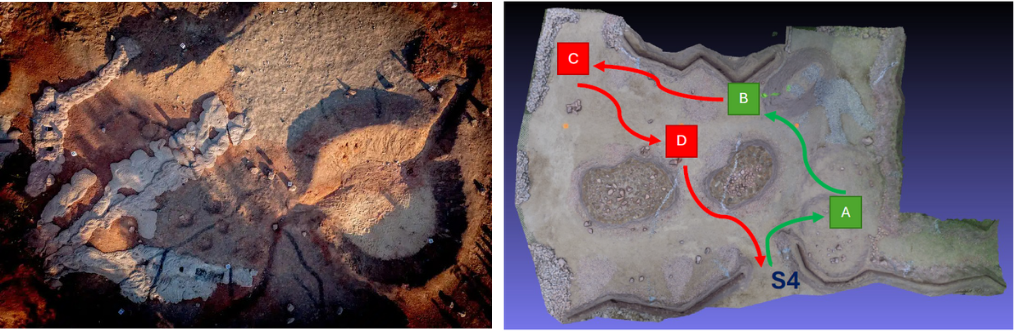
\includegraphics[width=85mm]{Navigation.png}}
    \caption{Constructed Mars Yard at the European Rover Challenge \cite{ERC}}
    \label{nav}
    \end{figure}
\begin{itemize}
    \item \textbf{Navigation Task:} 
    This task challenges the system’s ability for semi to fully autonomous navigation on a constructed Mars yard as illustrated in Fig. \ref{nav}. The rover is intended to navigate the uneven terrain consisting of rocks, trenches, etc. The remote communication system is required to operate the rover from a base station 100m apart at its maximum in the presence of multiple networks and occlusions. Furthermore, the rover base is supposed to navigate in the yard for 60 minutes. The rover is provided with 4 waypoints on the Mars yard [A-B-C-D] as shown in Fig. \ref{nav} and is required to navigate to them and return back to its start location. \cite{ERC} 
    
    \item \textbf{Surface Sampling Task:} The main goal of this sub-task is to collect surface samples of the constructed Martian soil and store it onboard for analysis. The samples include rocks, sand, etc. The rover is supposed to navigate to the location similar to the navigation task. To collect the surface samples, the rover is intended to employ a manipulator. \cite{ERC} 
    
    \item \textbf{Deep Sampling Task:} For this task, the rover is supposed to collect the soil samples from 30 cm below the Martian surface. The task requires to employ a sample collection device capable of drilling 30 cm below the constructed Martian Surface and collected at least 100 grams of the soil sample. The soil profile is stratified and visually coded with distinct colors at varying depths as illustrated in Fig. \ref{deepsample}. \cite{ERC} A telescopic drill design is developed for this task and is employed on the rover base. 

    \begin{figure}[htbp]
    \centerline{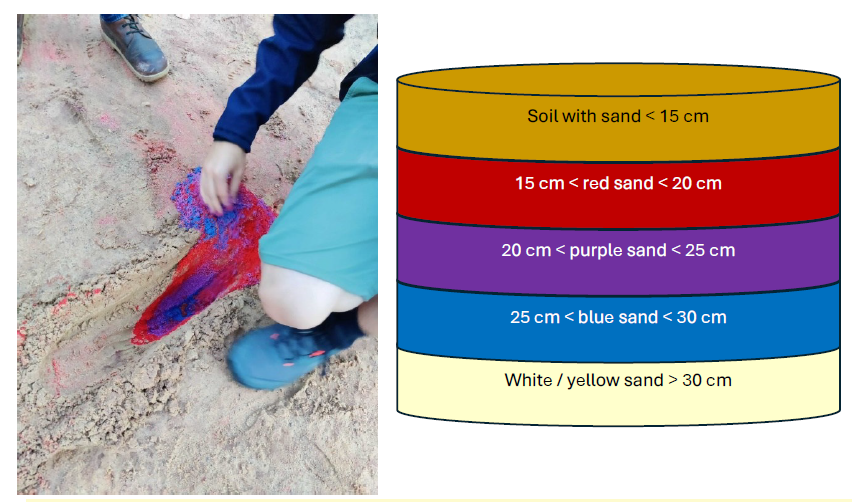
\includegraphics[width=65mm]{Deep_sample.PNG}}
    \caption{Coloured Soil Profile for Deep Sampling \cite{ERC}}
    \label{deepsample}
    \end{figure}
\end{itemize}

In order to tackle the tasks described, this paper provides the mechanical design of the rover base, arm and drill in Section IV. The electrical architecture to operate the rover and its components for the specified mission times is explained in Section V. Furthermore, the communication architecture required to operate the rover remotely is detailed in Section VI. The complete setup is illustrated in Fig. \ref{}. 



\label{sec:mech:base}

% ===================== Parameters (edit numbers only) ========================
\newcommand{\rWheel}{\SI{0.120}{\meter}}      % wheel radius (Ø240 mm)
\newcommand{\wWidth}{\SI{0.070}{\meter}}      % wheel face width (70 mm)
\newcommand{\Ttrack}{\SI{0.642}{\meter}}      % track width
\newcommand{\cBogie}{\SI{0.283}{\meter}}      % adjacent wheel spacing
\newcommand{\Lspan}{\SI{0.566}{\meter}}       % front--rear contact span (~2c)
\newcommand{\gcbelly}{\SI{0.215}{\meter}}     % belly clearance (level ground, current CAD)
\newcommand{\gcrear}{\SI{0.147}{\meter}}      % rear clearance (lowest: drill)
\newcommand{\Orrear}{\SI{0.209}{\meter}}      % rear overhang to lowest point
\newcommand{\hCOM}{\SI{0.282}{\meter}}        % CoM height from CAD
\newcommand{\Wfull}{\SI{706.3}{\newton}}      % total weight (~72 kg, Earth)
\newcommand{\Lcross}{\SI{0.525}{\meter}}      % H-diff crossbar span
\newcommand{\ltie}{\SI{0.272}{\meter}}        % tie-rod free length (adjustable)
\newcommand{\abell}{\SI{0.045}{\meter}}       % bellcrank arm (pivot->rod pin)
\newcommand{\Reff}{\SI{0.25}{\meter}}         % rocker effective lever arm
\newcommand{\drod}{\SI{19}{\milli\meter}}     % tie-rod diameter (solid Al)
\newcommand{\Etie}{\SI{70}{\giga\pascal}}     % EN-AW 5754 Young's modulus
\newcommand{\sigyHoneone}{\SI{80}{\mega\pascal}}  % 5754-H111 yield (typ.)
\newcommand{\sigyHtwoTwo}{\SI{160}{\mega\pascal}} % 5754-H22 yield (typ.)
\newcommand{\Sy}{2.5}                         % yield safety factor
\newcommand{\gammabuck}{2.0}                  % buckling safety factor
% Drive module (per wheel)
\newcommand{\tauWheel}{\SI{5}{\newton\meter}} % motor torque (per wheel)
\newcommand{\rpmMax}{\SI{110}{\minute^{-1}}}   % max wheel speed (rev/min)

% ========================= Figure 1: Overview (robust to missing file) ======

    \begin{figure}[htbp]
    \centerline{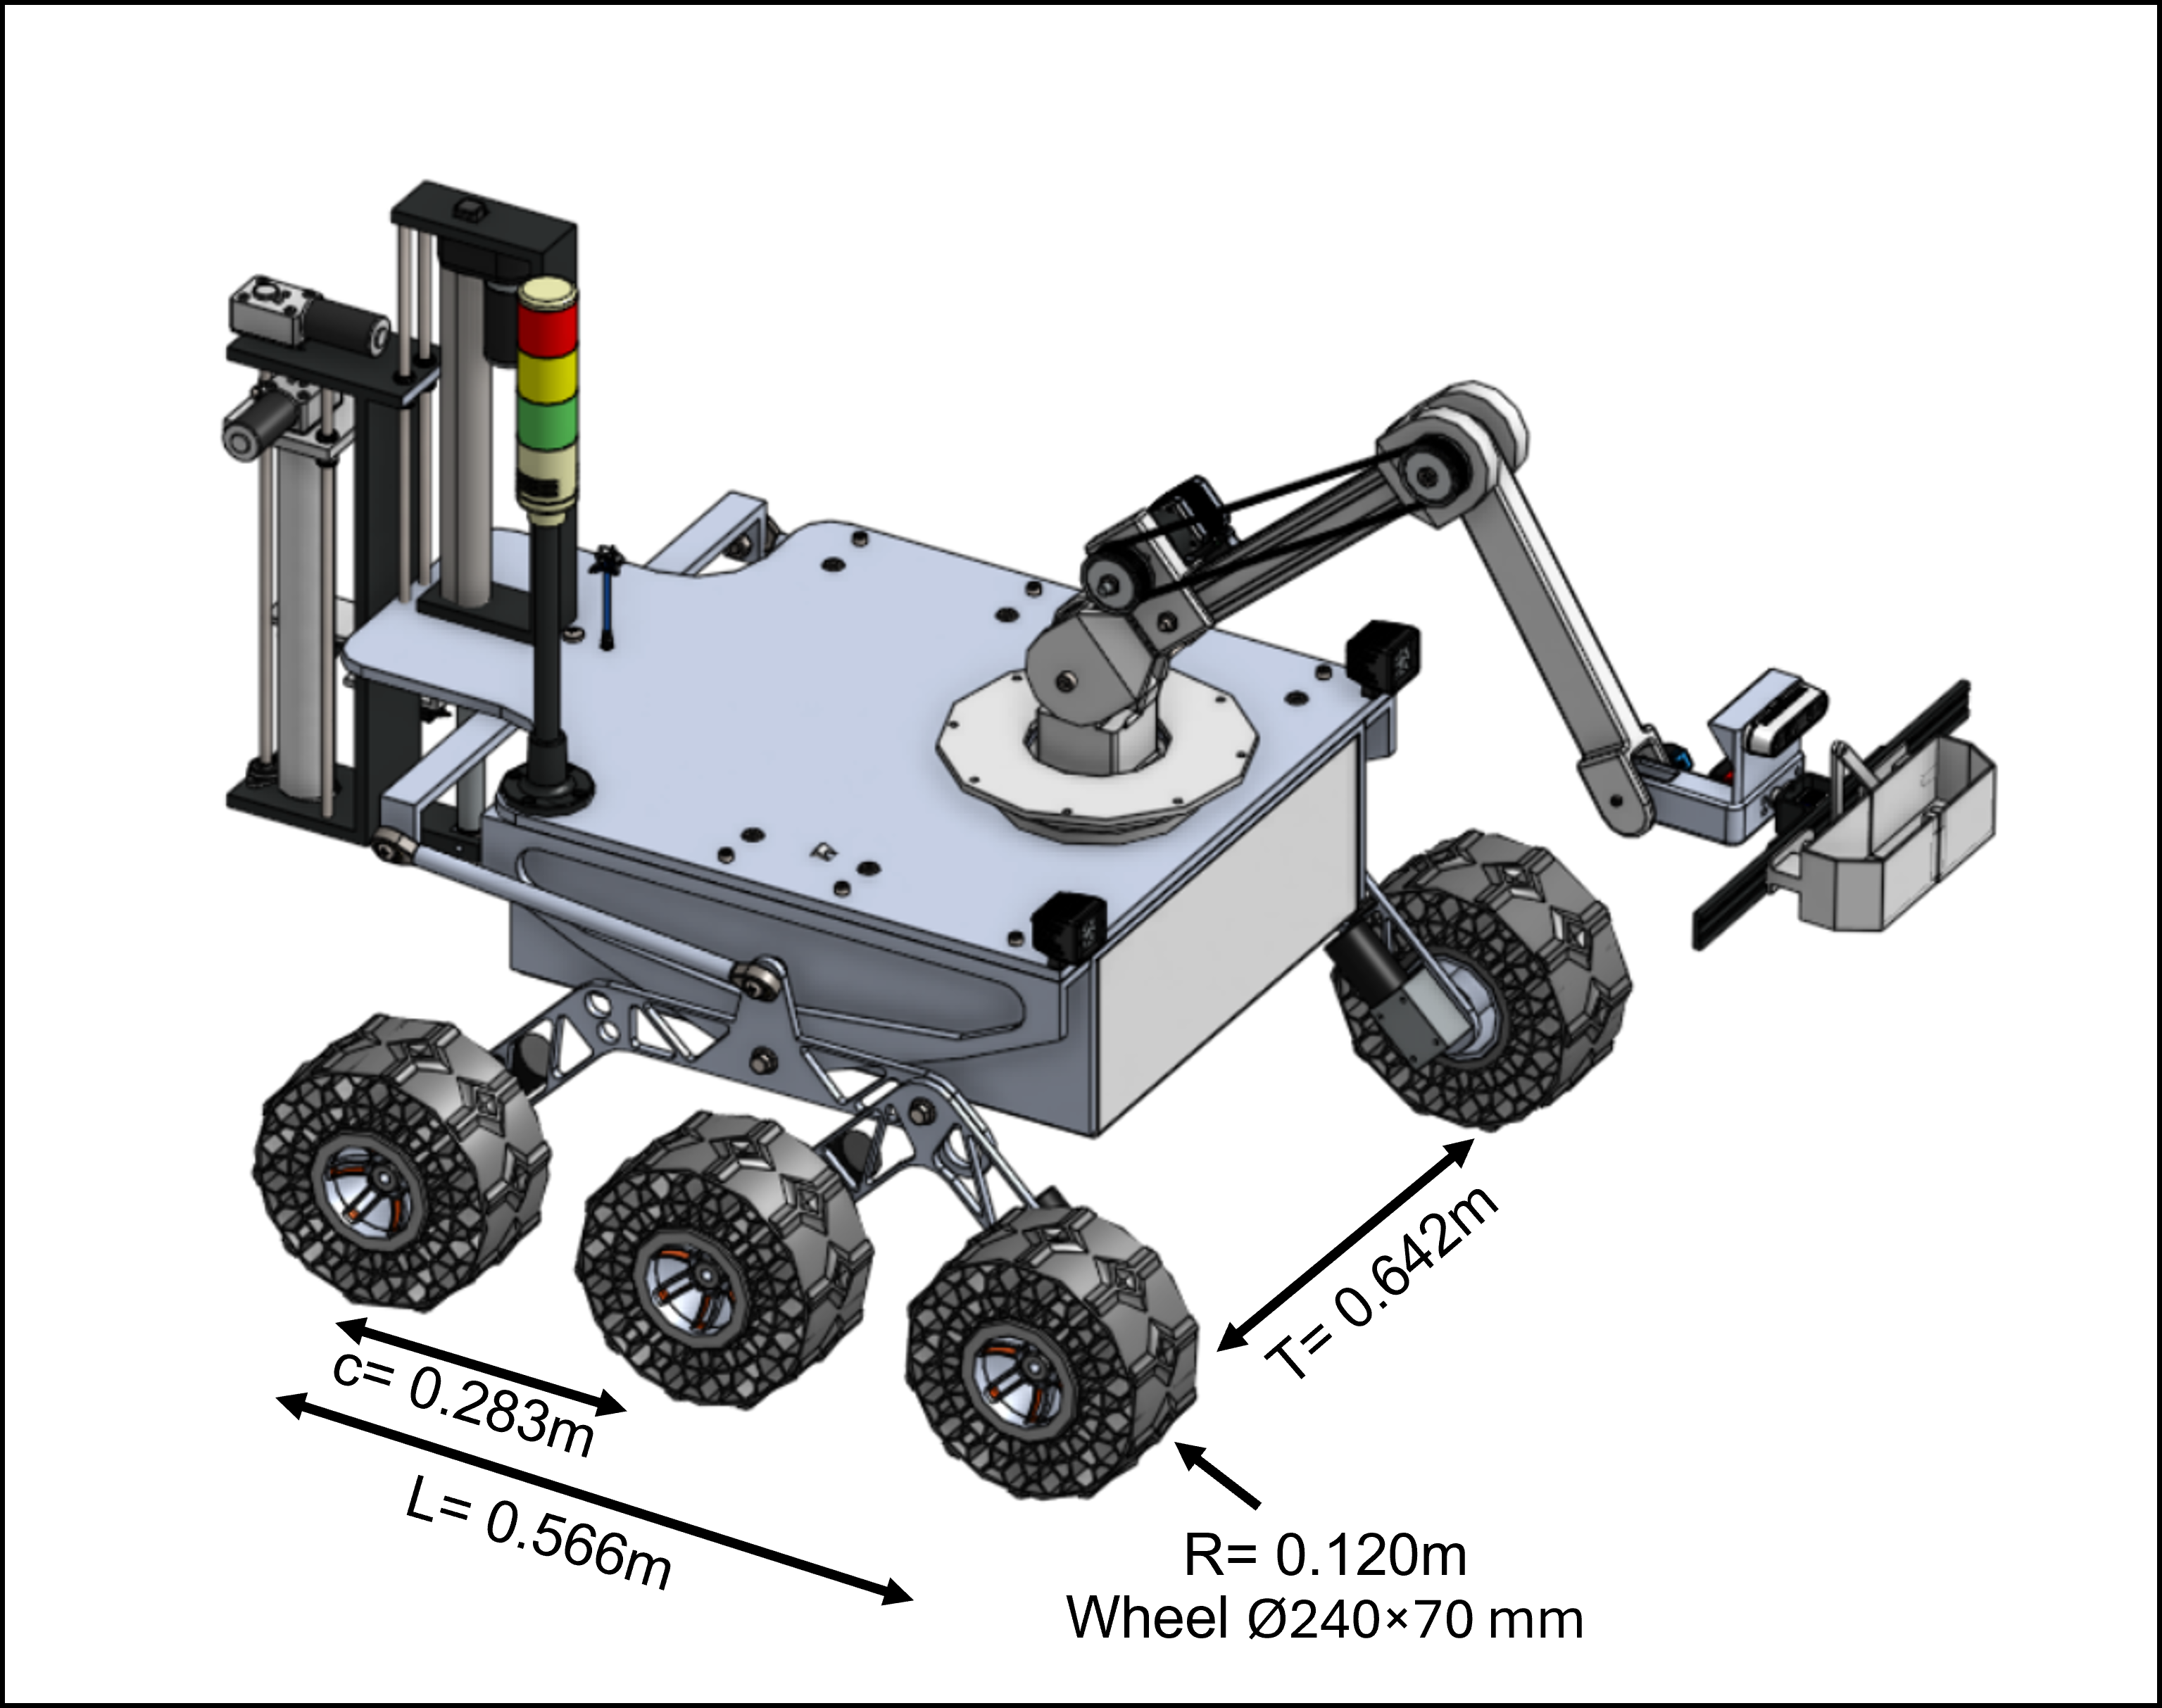
\includegraphics[width=80mm]{figures/rover_iso.png}}
    \caption{Rover with rocker--bogie mechanism, a horizontal differential and TPU wheels}
    \label{fig:rover_iso}
    \end{figure}

\section{MECHANICAL DESIGN}
\subsection{Rover Base Design}
The rover base uses a six-wheel rocker--bogie mechanism with a horizontal differential that averages left/right rocker motion. The topology preserves three contacts per side and passively redistributes load over uneven terrain, as developed on planetary rovers \cite{harrington2004,rivellini1993}. A horizontal differential reduces package height, eases sealing, and allows thread-based adjustment of the neutral ride height. Table~\ref{tab:geom} illustrates the geometric variables considered for the rover design. The kinematic envelope (\emph{angle of approach} \(\alpha_{\mathrm{app}}\), \emph{breakover angle} \(\beta_{\mathrm{brk}}\), \emph{angle of departure} \(\alpha_{\mathrm{dep}}\)) and obstacle bounds are derived using these variables. The geometric limits inform static tipover margins, which then combine with motor torque and traction models to bound gradeability and speed. Finally, the horizontal differential is justified and its tie-rods are sized before summarizing factors of safety and build choices.

% ========================= Geometry table ===================================
\begin{table}[htbp]
\caption{Measured geometry and drive parameters (level ground, Earth).}
\label{tab:geom}
\centering
\footnotesize
\begin{tabular}{l r}
\hline
Wheel radius $R$ & \rWheel \\
Wheel width $b$ & \wWidth \\
Track width $T$ & \Ttrack \\
Adjacent spacing $c$ & \cBogie \\
Front--rear span $L$ & \Lspan \\
Belly clearance $h_b$ & \gcbelly \\
Tail clearance $h_{\mathrm{tail}}$ & \gcrear \\
Rear overhang $O_r$ & \Orrear \\
CoM height $h_{\mathrm{COM}}$ & \hCOM \\
Weight $W$ (Earth) & \Wfull \\
Motor torque (per wheel) $\tau$ & \tauWheel \\
Max wheel speed $n_{\max}$ & \rpmMax \\
\hline
\end{tabular}
\end{table}

\subsubsection{Kinematic capacity and obstacle metrics}
This section determines the geometric envelope before adding dynamics/traction.  
\(\alpha_{\mathrm{app}}\) and \(\alpha_{\mathrm{dep}}\)  are the largest ramp angles the rover can achieve without a structural strike. Whereas breakover angle \(\beta_{\mathrm{brk}}\) is the maximum crest angle that avoids belly-ground contact.

\paragraph*{Approach angle}
During approach, the rover presents a wheel-first profile with no forward appendage below axle height, arm rotated aft; consequently, the front rim bounds the approach angle, hence:
\begin{equation}
\alpha_{\mathrm{app}}\approx \ang{90}
\end{equation}

\paragraph*{Breakover and departure angle}
Breakover angle (belly clearance \(h_b\) over span \(L\)) is calculated as follows:
\begin{equation}
\beta_{\mathrm{brk}}=2\arctan\!\Big(\frac{2h_b}{L}\Big)
=2\arctan\!\Big(\frac{2\times 0.215}{0.566}\Big)=\ang{74.45}
\end{equation}
Whereas, the Departure angle (for tail clearance \(h_{\mathrm{tail}}\) and rear overhang \(O_r\)) is calculated as:
\begin{equation}
\alpha_{\mathrm{dep}}=\arctan\!\Big(\frac{h_{\mathrm{tail}}}{O_r}\Big)
=\arctan\!\Big(\frac{0.147}{0.209}\Big)=\ang{35.15}
\end{equation}

\paragraph*{Step and ditch bounds.}
For a vertical step of height \(h\), the bogie must rotate \(\phi_{\mathrm{req}}=\arcsin(h/c)\). 
With \(h=R=\SI{0.120}{m}\),
\begin{equation}
\phi_{\mathrm{req}}=\arcsin\!\Big(\frac{0.120}{0.283}\Big)=\ang{25.1}
\end{equation}
Given \(\phi_{\max}\approx \ang{30}\), the kinematic step bound is
\begin{equation}
h_{\mathrm{step,max}}=\min\{R,\;c\sin\phi_{\max}\}=\min\{0.120,\;0.141\}=\SI{0.120}{m}
\end{equation}
For a rectangular ditch with no sidewall contact:
\begin{equation}
\begin{aligned}
w_{\max} &\approx L - 2\sqrt{(R+h_b)^2 - h_b^2}\\
         &= \SI{0.052}{\meter}\quad\text{(\SI{0.05}{m} is adopted as a design limit)}
\end{aligned}
\end{equation}
Here $w_{\max}$ denotes the largest rectangular ditch (vertical walls) that can be
spanned with the front and rear wheels resting on the two edges while maintaining at
least the belly clearance $h_b$ (no sidewall contact, neutral stance, no sinkage).
Geometrically, a line at height $h_b$ above the ground must remain \emph{tangent} to
each wheel of radius $R$ which occurs at a horizontal offset
$d=\sqrt{(R+h_b)^2-h_b^2}=\sqrt{R(R+2h_b)}$ from each wheel–ground contact.
Therefore the allowable gap is the remaining span between these two offsets which evaluates to $\SI{0.052}{m}$.

\subsubsection{Static stability}\label{subsec:static-stability}

Geometric clearances do not guarantee against overturning which can lead to tipover. Hence, this subsection calculates the static stability of the rover.  
With \(b_y=T/2\) and \(b_x=L/2\) and fixed \(h_{\mathrm{COM}}\). The max roll angle and max pitch angle are as follows:
\begin{equation}
\begin{aligned}
\theta_{\mathrm{roll,tip}}  &= \arctan\!\Big(\tfrac{b_y}{h_{\mathrm{COM}}}\Big) = \ang{48.7}\\
\theta_{\mathrm{pitch,tip}} &= \arctan\!\Big(\tfrac{b_x}{h_{\mathrm{COM}}}\Big) = \ang{45.1}
\end{aligned}
\end{equation}
The broader TPU (Thermoplastic polyurethane) tread does not change these geometric limits but increases lateral shear reserve and reduces sinkage, postponing loss of support that typically precedes geometric tipover.

% --- Heading has math: give hyperref a plain-text PDF string to avoid warnings
\paragraph*{Motor, torque, and speed caps}
This section analyzes and translates geometry into attainable slopes/speeds and specifies actuation limits. Each wheel uses an ODrive BotWheel BLDC module. The nominal per-wheel torque in Table~\ref{tab:geom}
($\tau=\SI{5}{N\,m}$) matches the vendor’s continuous rating using the documented
torque constant $K_t=\SI{0.951}{N\,m/A}$ and continuous current $I_{\mathrm{cont}}=\SI{5}{A}$ (free air),
giving $\tau_{\mathrm{cont}}\approx \SI{4.8}{N\,m}$. The wheel speed is software-capped at $n_{\max}=\SI{110}{\minute^{-1}}$ via the ODrive velocity deliberately to preserve the traction margin and stay within the motor/controller thermal envelope. With speed constant $K_v=\SI{8.7}{\rpm\volt^{-1}}$ and DC bus voltage $V_{\mathrm{bus}}=\SI{24}{\volt}$, the no-load speed is
$n_0\approx K_v V_{\mathrm{bus}}\approx \SI{209}{\minute^{-1}}$. Approximating the motor with a linear
torque–speed slope $S_{n\tau}=\SI{10.98}{\rpm\newton^{-1}\metre^{-1}}$ (vendor fit),
the rated-load speed ($n$) at $\tau=\SI{5}{N\,m}$ is
\[
\begin{aligned}
n &\approx n_0 - S_{n\tau}\,\tau \approx \SI{155}{\minute^{-1}}                        \cite{odriveBotwheelDocs,odriveBotwheelsShop}
\end{aligned}
\] 




\paragraph*{Traction, gradeability, and speed \texorpdfstring{ (For TPU, \(\tau=\SI{5}{N\,m}\) and \(n_{\max}=\SI{110}{\minute^{-1}}\))}{(TPU, tau=5 N m, n\_max=110 min^{-1})}} With \(\theta_{\mathrm{tip}}\) and actuation fixed, the torque and traction is combined.  
Here, \(n_{\max}=\SI{110}{\minute^{-1}}\) is forced in the controller and the No-slip top speed (v\_max) uses this cap:
\begin{equation}
v_{\max}=\frac{2\pi n_{\max} R}{60}
=\frac{2\pi(110)(0.120)}{60}=\SI{1.38}{m/s}
\end{equation}
Drive force with torque limitation for six wheels is as follows:
\begin{equation}
F_{\mathrm{drive}}=\frac{6\tau}{R}
=\frac{6\times\SI{5}{N\,m}}{\SI{0.120}{m}}=\SI{250}{N}
\end{equation}
The grade requirement is \(W\sin\theta\le \min\{F_{\mathrm{drive}},\,\mu W\}\), which yields:
\begin{equation}
\theta_{\max} = \min\Big\{\arcsin\!\Big(\frac{F_{\mathrm{drive}}}{W}\Big),\;\arctan\mu,\;\theta_{\mathrm{pitch,tip}}\Big\}
\end{equation}
\paragraph*{Traction model and units}
Let $\mu$ denote the \emph{effective longitudinal wheel--ground friction coefficient} (dimensionless).
The traction bound is $F_{\text{traction}}^{\max}=\mu W \Rightarrow W\sin\theta \le \mu W$, so the
\emph{traction-limited slope angle} is
\[
\theta_\mu=\arctan(\mu)
\]

In this work we sweep $\mu\in\{0.6,0.8,1.0\}$ to represent loose sand, compacted soil, and firm ground/rock.


At $W=\SI{706}{N}$ the torque limit is $\arcsin(250/706)=\ang{20.7}$, i.e., about $38\%$ grade. In eq [], for $\mu\in\{0.6,0.8,1.0\}$, $\theta_\mu$ is 
$\{\ang{31.0},\,\ang{38.7},\,\ang{45.0}\}$, which correspond to
$\{60\%,\,80\%,\,100\%\}$ grade (since $G=100\tan\theta$, at the traction limit $G=100\mu$).
Therefore, the rover climb is torque-limited to \textbf{\ang{20.7}} ($\sim$38\% grade) unless gearing or motor torque is raised.




% ========================= Figure: Bekker sweep (robust to missing file) =====
    \begin{figure}[htbp]
    \centerline{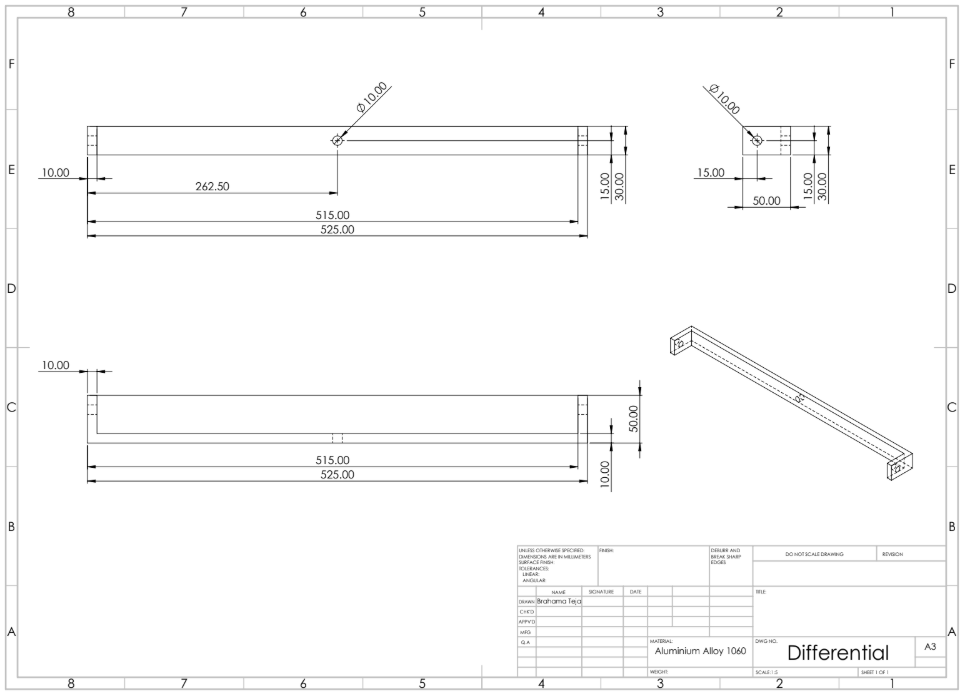
\includegraphics[width=80mm]{figures/hdiff_layout.png}}
    \caption{Engineering drawing of the horizontal differential \textbf{crossbar}
(overall length \(\Lcross\)); orthographic and isometric views with key
dimensions. Bellcranks and tie-rods are not shown in this sheet.}
    \label{fig:hdiff}
    \end{figure}


\subsubsection{Horizontal differential}
To keep body attitude within tip margins on cross-slope terrain while maintaining passive compliance, the \emph{kinematics and effects} of the horizontal differential are studied in this subsection. The mechanism comprises a crossbar of width \(\Lcross\) and two equal-arm bellcranks of arm \(a_b=\abell\) on the rockers, connected by adjustable rods of free length \(\ell_t=\ltie\) and diameter \(\varnothing\drod\). Linearized about neutral
\begin{equation}
\Delta \ell_L \approx -a_b\,\theta_L,\qquad
\Delta \ell_R \approx -a_b\,\theta_R
\end{equation}
Here, the compatibility is required to satisfy \(\theta_L+\theta_R \approx 0\), so the chassis attitude follows the \emph{average} terrain slope \cite{rivellini1993}.

Figure~\ref{fig:hdiff} shows the engineering drawing of the \emph{horizontal differential crossbar}. The crossbar spans \Lcross\ between the rocker pivots and defines the mounting/datum geometry for the mechanism. Equal-arm bellcranks and the adjustable links are not shown in this sheet. They attach at the end hole pattern on the crossbar and, together, enforce \(\theta_L+\theta_R\approx 0\) so that the body follows the average terrain slope as derived above.




\begin{table}[htbp]
\caption{H-diff tie-rod: results and sensitivity (the ranges correspond to assembly tolerances).}
\label{tab:tierod}
\centering
\footnotesize
\begin{tabular}{p{0.64\columnwidth} >{\raggedleft\arraybackslash}p{0.30\columnwidth}}
\hline
Axial load $F_t$ from \eqref{eq:Ft} & \SI{0.981}{kN} \\
Strength FS (5754-H111 / H22) & $7.4\ / \ 14.8$ \\
Euler buckling FS ($\gamma\!=\!2$) & $30.4$ \\
Body-roll leak $\theta_{\mathrm{body}}$ & \ang{0.000385} \\
\hline
\multicolumn{2}{p{\dimexpr0.94\columnwidth}}{\textit{Sensitivity:} $R_{\!eff}\in[\SI{0.22}{m},\SI{0.28}{m}]$, $a_b\in[\SI{0.040}{m},\SI{0.055}{m}]$} \\
$F_t$ range & \SIrange{0.706}{1.236}{kN} \\
Min strength FS (H111) across range & $>6.0$ \\
Min buckling FS across range & $>24$ \\
\hline
\end{tabular}
\end{table}
% ========================= Figure: H-diff layout (robust to missing file) ====


\subsubsection{Tie-rod sizing}
To improve the strength, buckling, stiffness and sensitivity of the tie-rod, the members carrying the differential loads are sized. The calculations are provided in this subsection. A conservative estimate puts approximately \(W/4\) on the front wheel; the moment \((W/4)\Reff\) reacted by a bellcrank of arm \(a_b\) gives the axial tie-rod force: 
\begin{equation}
\boxed{F_t=\dfrac{W\,\Reff}{4a_b}}
=\frac{(706.3)(0.25)}{4(0.045)}=\SI{981}{\newton}
\label{eq:Ft}
\end{equation}

\paragraph*{Strength.}
Net threaded-end area \(A_{\text{net}}=\tfrac{\pi}{4}(D^2-d_{\mathrm{tap}}^2)=\SI{226.8}{\milli\meter^2}\) (with \(D=\SI{19}{mm}\), M10 tap drill \(d_{\mathrm{tap}}=\SI{8.5}{mm}\)).
Allowables are \((\sigma_y/S_y)A_{\text{net}}\):
\[
\text{FS}_{\text{strength}}=
\begin{cases}
\dfrac{(80/2.5)A_{\text{net}}}{981}=\mathbf{7.4} & \text{(5754-H111)}\\[4pt]
\dfrac{(160/2.5)A_{\text{net}}}{981}=\mathbf{14.8} & \text{(5754-H22)}
\end{cases}
\]

\paragraph*{Buckling.}
With \(I=\pi D^4/64=\SI{6.40e-9}{m^4}\) and \(L=\ell_t=\SI{0.272}{m}\),
\[
P_{\mathrm{cr}}=\frac{\pi^2 E I}{L^2}
=\SI{59.7}{\kilo\newton},\qquad
\text{FS}_{\text{buck}}=\frac{P_{\mathrm{cr}}/\gamma}{F_t}=\mathbf{30.4}
\]


\paragraph*{Stiffness (body-roll leak).}
Axial stiffness \(k_a=EA/L\) with cross section area \(A_{\text{solid}}=\pi D^2/4=\SI{2.835e-4}{m^2}\) gives \(k_a=\SI{7.3e7}{N/m}\).
The chassis roll leak under differential action is
\[
\boxed{\theta_{\mathrm{body}}=\frac{W \Reff}{8 a_b}\frac{L}{E A_{\text{solid}}}}
=\ang{0.000385}
\]
Table~\ref{tab:tierod} condenses the design checks for the \emph{tie-rods}, i.e., the most highly loaded members in the horizontal differential load path. It reports:
(i) the axial load \(F_t\) from the worst-case quasi-static cross-slope moment balance (derived in \eqref{eq:Ft});
(ii) strength safety factors for EN~AW-5754 in two tempers (H111/H22);
(iii) Euler buckling safety factor using end-condition \(\gamma=2\);
and (iv) the small-angle body-roll “leak” \(\theta_{\mathrm{body}}\) predicted from the \emph{axial stiffness of the rod alone}.
The sensitivity block varies \(R_{\!eff}\) and \(a_b\) over realistic assembly tolerances and shows that \(F_t\) remains within \(\SIrange{0.706}{1.236}{kN}\) while \(\mathrm{FS}_{\text{strength}}>6\) and \(\mathrm{FS}_{\text{buck}}>24\) are preserved. 
\emph{Interpretation:} the tie-rods are not a limiting component for either strength or stability; margins remain comfortable across tolerances. The quoted \(\theta_{\mathrm{body}}\) is a \textbf{lower bound} (rod-stiffness only) and ignores bellcrank/crossbar flex and joint/frame compliance.

\begin{table}[htbp]
        \centering
        \footnotesize
        \caption{Static tipover margins.}
        \label{tab:stability_fos}
        \begin{tabular}{@{}lccc@{}}
        \hline
        Required slope $\theta_{\mathrm{req}}$ & \ang{30} & \ang{35} & \ang{40} \\
        \hline
        Roll tip margin $\mathrm{FS}_{\mathrm{tip,roll}}$ & 1.98 & 1.63 & 1.36 \\
        Pitch tip margin $\mathrm{FS}_{\mathrm{tip,pitch}}$ & 1.73 & 1.43 & 1.19 \\
        \hline
        \end{tabular}
\end{table}    


\subsubsection{Factors of Safety}
Let $\theta$ denote the ground slope angle.
$\theta_{\mathrm{req}}$ is the \emph{required} slope for a scenario.
$\theta_{\mathrm{tip}}$ is the \emph{static tipover angle} about the relevant axis
(roll for cross-slope, pitch for uphill), computed in
Sec.~\ref{subsec:static-stability}:
$\theta_{\mathrm{tip,roll}}=\ang{48.7}$, $\theta_{\mathrm{tip,pitch}}=\ang{45.1}$.
All angles are in degrees; the safety-factor ratio below is unitless. The geometry, actuation, and member sizing is rolled into pass/fail margins.  
An FoS $\ge 1$ is considered pass for the given condition.
\begin{itemize}
    \item \textbf{Static tipover margins (geometry-only):} Define \(\mathrm{FS}_{\mathrm{tip}}(\theta_{\mathrm{req}})=\tan(\theta_{\mathrm{tip}})/\tan(\theta_{\mathrm{req}})\).
    

\begin{table}[htbp]
\centering
\footnotesize
\caption{Torque FoS on Earth ($W=\SI{706}{N}$)}
\label{tab:torque_fos}
\begin{tabular}{@{}lcccc@{}}
\hline
$\theta$ & \ang{15} & \ang{20} & \ang{25} & \ang{30} \\
\hline
Earth $\mathrm{FS}_{\tau}$ & 1.37 & 1.03 & 0.84 & 0.71 \\

\hline
\end{tabular}
\end{table}


\item \textbf{Drive torque margins:}
Table \ref{tab:torque_fos} illustrates the drive torque FOS on Earth. The drive torque is calculated by:

\(\mathrm{FS}_{\tau}(\theta)=F_{\mathrm{drive}}/(W\sin\theta)\) with \(F_{\mathrm{drive}}=\SI{250}{N}\)


\begin{table}[htbp]
\centering
\footnotesize
\caption{Traction FoS for $\mu \in \{0.60, 0.80\}$.}
\label{tab:traction_fos}
\begin{tabular}{@{}lcccc@{}}
\hline
$\theta$ & \ang{20} & \ang{25} & \ang{30} & \ang{35} \\
\hline
$\mu=0.60$ & 1.65 & 1.29 & 1.04 & 0.86 \\
$\mu=0.80$ & 2.20 & 1.72 & 1.39 & 1.14 \\
\hline
\end{tabular}
\end{table}



\item \textbf{Traction FOS wrt Friction:}
Table \ref{tab:traction_fos} illustrates the Traction FOS for different values of friction. The FOS is calculated as follows:
\begin{equation}
\mathrm{FS}_{\mu}(\theta) = \frac{\mu}{\tan\theta}
\label{eq:FS_mu}
\end{equation}


\item \textbf{Robustness Reading:}
From Table \ref{tab:stability_fos}, at \ang{30}, roll tip and pitch tip margins are \(\mathrm{FS}_{\mathrm{tip,roll}}\!\approx\!1.98\), \(\mathrm{FS}_{\mathrm{tip,pitch}}\!\approx\!1.73\), \(\mathrm{FS}_\mu\!\in[1.04,1.39]\), and tie-rod strength/buckling FoS of \(>\!7\) and \(>\!30\), respectively.
\end{itemize}
\subsubsection{Material and manufacturing notes}
EN~AW-5754 (Al--Mg3) is chosen for plates and tie-rods for corrosion resistance, specific stiffness, and availability. Typical proof strengths (H111: \SIrange{60}{80}{\mega\pascal}, H22: \SIrange{130}{185}{\mega\pascal}) provide comfortable margins for the computed loads \cite{tk5754,rb5754h111,tk5754h22}. Rocker and bogie plates are laser-cut from sheet at \(t=\SI{8}{\milli\meter}\), with local ribbing to maintain section modulus near bearings and motor mounts. Brackets/flanges are press-bent on a hydraulic press where required. The minimum inside bend radius is respected according to the guideline: \(r_i\!\gtrsim\!1.0t\) for H111 and \(r_i\!\gtrsim\!1.5t\) for H22 with bend-relief slots to manage strain and edge pull. Torque specifications conform to ISO classes for carbon-steel fasteners (e.g., 8.8/10.9), with thread-locking compound on non-reversible joints.


\subsection{Robotic Arm Design}
This subsection introduces the 5 DOF robotic arm which is particularly designed based on the requirements of the sampling task in the ERC. A custom gripper to satisfy the surface sample collecting task is designed to collect rocks and soil samples. It acts as traditional 2 finger end effector and sample collecting end effector. The arm is mounted on the rover and this will coordinate with it during its operation. The motors are selected based on the results of torque calculations at each joint. In order to keep under the marginal weight, standard aluminium extrusion rods and 3D printed joints are used in the design. Denavit-Hartenberg (DH) parameters are used to determine the forward kinematics. For inverse kinematics, algebraic solution is used to define the position and orientation of the end effector.

\subsubsection{Forward Kinematics}
Forward kinematics delineates the process of ascertaining the position and orientation of a manipulator's end-effector from the robot's joint variables. This computational mapping from the joint space to the Cartesian space is foundational for the precise control and simulation of robotic movements. A standardized methodology for this process is the Denavit-Hartenberg (DH) [] convention, which offers a systematic approach to assigning coordinate frames to each link in a kinematic chain. Instead of the six parameters typically required to define a rigid body's spatial configuration, the DH method employs only four: link length, link twist, link offset, and joint angle $(di, ai, θi, and αi)$. These parameters comprehensively describe the geometric relationship between consecutive link frames. This condensed set of parameters is then utilized to formulate a homogeneous transformation matrix. This 4x4 matrix illustrated in eq.[] mathematically encapsulates the rotation and translation between adjacent coordinate frames. By sequentially multiplying the individual transformation matrices from the base of the manipulator to its endpoint, the cumulative transformation is de-rived. This resultant matrix provides the precise Cartesian coordinates and orientation of the end-effector relative to the robot's base frame. Each transformation matrix using DH parameters is calculated as follows:
\begin{equation}
T_i = R_{z,\theta_i} \; T_{z,d_i} \; T_{x,a_i} \; R_{x,\alpha_i}
\end{equation}
\begin{equation}
T_i = 
\begin{bmatrix}
\cos\theta_i & \sin\theta_i \cos\alpha_i & \sin\theta_i \sin\alpha_i & a_i \cos\theta_i \\
\sin\theta_i & \cos\theta_i \cos\alpha_i & \cos\theta_i \sin\alpha_i & a_i \sin\theta_i \\
0 & \sin\alpha_i & \cos\alpha_i & d_i \\
0 & 0 & 0 & 1
\end{bmatrix}
\end{equation}
where:
\begin{flalign*}
& P_x = a_i \cos\theta_i &
& P_y = a_i \sin\theta_i &
& P_z = d_i & \\
& a_i : \text{ Link length} &
& \alpha_i : \text{ Link twist} & 
& d_i : \text{ Link offset} & \\
& \theta_i : \text{ Joint angle} & 
\end{flalign*}


The parameters considered for designing the 5 DOF robotic arm are listed in Table 1 which shows rotation about the z-axis αᵢ, rotation about the x-axis (θᵢ), transition along the z-axis (aᵢ), and transition along the x-axis (dᵢ). By substituting the D-H parameters of Table~\ref{tab:dh} into Eq (), the individual transformation matrices T⁰₁ to T⁴₅, and a global matrix of transformation T⁰₅ are obtained as per []:

\begin{table}[h!]
\centering
\renewcommand{\arraystretch}{1.2}
\begin{tabular}{|c|c|c|c|c|}
\hline
Link & $a_i$ (mm) & $\alpha_i$ (deg) & $d_i$ (mm) & $\theta_i$ (deg) \\
\hline
1 & 0   & 90 & 210   & $\theta_1$ \\
2 & 425 & 0  & 0     & $\theta_2$ \\
3 & 400 & 0  & 0     & $\theta_3$ \\
4 & 0   & 90 & 0     & $\theta_4$ \\
5 & 0   & 0  & 260 & $\theta_5$ \\
\hline
\end{tabular}
\caption{DH parameters for the 5 DOF robotic arm}
\label{tab:dh}
\end{table}
The position and orientation of the wrist is determined by successive multiplying of the transformation matrices:
\begin{align}
T^0_3 &= T^0_1 T^1_2 T^2_3 \\
T^3_5 &= T^3_4 T^4_5\\
T^0_5 &= T^0_3 T^3_5
\end{align}

The resulting overall transformation is:
\begin{equation}
T^0_5 =
\begin{bmatrix}
n_{11} & n_{12} & n_{13} & n_{14} \\
n_{21} & n_{22} & n_{23} & n_{24} \\
n_{31} & n_{32} & n_{33} & n_{34} \\
0 & 0 & 0 & 1
\end{bmatrix}
\end{equation}
where each $n_{ij}$ is a function of the joint parameters as per [].

\subsubsection{Inverse Kinematics}

Inverse kinematics for the 5 DOF arm are derived algebraically as per the relation:
\begin{equation}
[T^0_1]^{-1} T^0_5 = [T^0_1]^{-1} T^0_3 T^3_4 T^4_5
\end{equation}

Expands to:
\begin{equation}
\begin{bmatrix}
c_1 n_{11} + s_1 n_{21} & c_1 n_{12} + s_1 n_{22} & c_1 n_{13} + s_1 n_{23} & c_1 x + s_1 y \\
 -s_1 n_{11} + c_1 n_{21} & -s_1 n_{12} + c_1 n_{22} & -s_1 n_{13} + c_1 n_{23} & -s_1 x + c_1 y \\
n_{31} & n_{32} & n_{33} & z - d_1 \\
0 & 0 & 0 & 1
\end{bmatrix}

\\= 
\begin{bmatrix}
\alpha_{11} & \alpha_{12} & \alpha_{13} & \alpha_{14} \\
\alpha_{21} & \alpha_{22} & \alpha_{23} & \alpha_{24} \\
\alpha_{31} & \alpha_{32} & \alpha_{33} & \alpha_{34} \\
0 & 0 & 0 & 1
\end{bmatrix}
\end{equation}

Each $\alpha_{i,j}$ is formed from the combination of sines and cosines of various joint angles (and DH parameters) resulting from the product of the transformation matrices as per [].
Therefore the joint angles are computed as follows:
\begin{flalign*}
& -s_1 x + c_1 y = 0 \implies \theta_1 = \text{atan2}(y, x) & \\
& \theta_2 = \text{atan2}(s_2, c_2) & \\
& \theta_3 = \text{atan2}(s_3, c_3) & \\
& \theta_4 = \theta_{234} - \theta_2 - \theta_3 & \\
& \theta_5 = \text{atan2}(s_5, c_5) &
\end{flalign*}
\subsubsection{Pre-determination of Joint Torques}

This section pre-determines the joint torques for the robotic arm for preliminary modelling of the robot arm. The whole robot arm assembly was divided into three subassemblies. The maximum length of subassembly 1 is a2 = 425 [mm] whereas that of subassembly 2 is a3 = 400 [mm] and of subassembly 3 is d5 = 260 [mm]. The centre of gravity for the subassemblies were considered to be placed in the middle of segments a2, a3 and d5. It was approximated that the maximum mass of the subassembly 1 is m1 = 1.33 [Kg] whereas that of the sub-assembly 2 is m2 = 0.32 [Kg] and for subassembly 3 is m3 = 1.0 [Kg];
\begin{itemize}
    \item The mass of the manipulated part si mp=1.0 [Kg];
    \item The total length of the robot is approximately Lt = 1085 [mm]; 
    \item The mass of the whole assembly is ms = 3.0 [Kg]
\end{itemize}
 
The determination of the joint toques T2, T3, T4 was performed for the following hypotheses where particular positions are presented in Fig. \ref{}


Joint torques for specific positions are as follows:
\begin{align*}
T_2  &= -[m_p g (a_2+a_3+d_5) + m_3 g (a_2+a_3+d_5/2) + m_2 g (a_2+a_3/2) + m_1 g (a_2/2)] \\
&= -24.624\ \mathrm{Nm} \\[1.5em]
T_3  &= -[ m_p g (a_3 + d_5) + m_3 g (a_3 + d_5/2) + m_2 g (a_3/2) ] \\
&\quad + 0.32 \times 9.81 \times (0.4/2) ] \\
&= -12.301\ \mathrm{Nm} \\[1.5em]
T_4  &= -[ m_p g d_5 + m_3 g (d_5/2) ] \\
&= -3.825\ \mathrm{Nm}
\end{align*}


\subsection{Drill Design}
This section details the design and analytical validation of a screw–auger drill intended to obtain deep samples of Martian regolith weighing \(\ge\)100~g per bore from a target depth of \(\,h_p=0.30~\mathrm{m}\) as mentioned in Section III. The mechanical design and soil context are explained in the following subsections followed by the derivation of the kinematics, axial thrust, and torque requirements, and transport capacity characteristics required for fulfilling the deep sampling task. The validation tables are provided at the end which demonstrate the selected actuator's compliance with the requirements. The drill comprises a TR8 lead screw for feed (down-thrust) and a solid flight auger for cuttings tr ansport. A  \emph{feed motor} applies torque to the lead screw to generate axial penetration. An independent \emph{auger motor} provides rotation to cut and convey regolith along the helical flute. The feed stage sets the axial velocity and the penetration time, while the auger stage determines the transport rate and torque draw. The drill design is illustrated in Fig.~\ref{drill}.
\begin{figure}[h!]
    \centering
    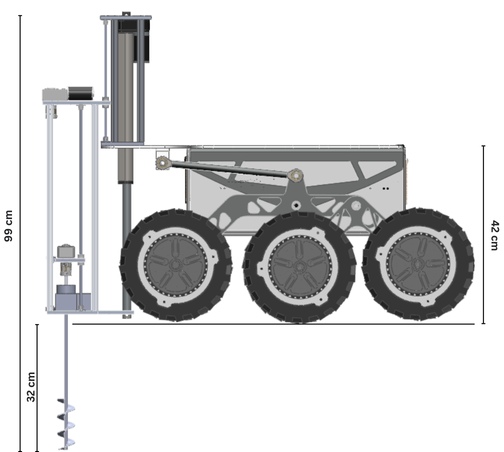
\includegraphics[width=0.75\linewidth]{drillcalc.png}
    \caption{}
    \label{drill}
\end{figure}

\subsubsection*{Design Parameters and Soil Assumptions}
Table~\ref{tab:design} lists the mechanical parameters used in analysis: auger geometry, motor ratings, and screw characteristics. The practical efficiencies of screw friction, \(\eta=0.35\), and thread friction, \(\mu=0.15\) (brass/steel), are used for the preliminary design.

\begin{table}[h!]
\centering
\caption{Design parameters  for auger drill system}
\label{tab:design}
\begin{tabular}{@{}llll@{}}
\toprule
\textbf{Symbol} & \textbf{Description} & \textbf{Value} & \textbf{Unit} \\
\midrule
\(D_a\) & Auger diameter & \(40\) & \(\mathrm{mm}\) \\
\(h_p\) & Target penetration depth & \(300\) & \(\mathrm{mm}\) \\
\(L_a\) & Physical auger length & \(420\) & \(\mathrm{mm}\) \\
\(\tau_a\) & Auger motor torque (rated) & \(1.765\) & \(\mathrm{N\cdot m}\) \\
\(n_a\) & Auger motor speed (rated) & \(50\) & \(\mathrm{rpm}\) \\
\(\tau_f\) & Feed motor torque (rated) & \(3.825\) & \(\mathrm{N\cdot m}\) \\
\(n_f\) & Feed motor speed (rated) & \(15\) & \(\mathrm{rpm}\) \\
\(l\) & Lead screw lead (TR8x2, 2-start) & \(4\) & \(\mathrm{mm/rev}\) \\
\(d_m\) & Lead screw mean diameter & \(8\) & \(\mathrm{mm}\) \\
\(L\) & Lead screw stroke length & \(420\) & \(\mathrm{mm}\) \\
\(p\) & Auger lead (pitch advance per rev) & \(12\) & \(\mathrm{mm}\) \\
\(\mu\) & Friction coefficient (screw, brass/steel) & \(0.15\) & \(-\) \\
\(\eta\) & Screw efficiency (practical) & \(0.35\) & \(-\) \\
\(g_{\oplus}\) & Gravity, Earth & \(9.81\) & \(\mathrm{m/s^2}\) \\
\bottomrule
\end{tabular}
\end{table}


These parameters size the kinematic advance (via \(l,n_f\)), determine the volumetric transport rate (\(D_a,p,n_a\)), and set the actuation capacity (\(\tau_f,\tau_a\)). The assumed efficiency \(\eta\) and friction \(\mu\) govern thrust conversion and back-drivability, respectively.

\begin{table}[h!]
\centering
\caption{Representative soil properties for Martian regolith layers}
\label{tab:soil}
\begin{tabular}{@{}llll@{}}
\toprule
\textbf{Symbol} & \textbf{Parameter} & \textbf{Value} & \textbf{Units} \\
\midrule
-- & Bulk density (surface sand) & \(1.1\) -- \(1.3\) & \(\mathrm{Mg/m^{3}}\) \\
-- & Bulk density (duricrust) & \(\sim 1.1\) & \(\mathrm{Mg/m^{3}}\) \\
-- & Bulk density (sand/gravel layer) & \sim 1.6 & \(\mathrm{Mg/m^{3}}\) \\
\(\rho\) & Soil bulk density (design) & \(1600\) & \(\mathrm{kg/m^{3}}\) \\
\(c\) & Soil cohesion (loose simulant) & \(1\) & \(\mathrm{kPa}\) \\
\(\phi\) & Soil friction angle & \(20\) & \(\mathrm{deg}\) \\
\bottomrule
\end{tabular}
\end{table}
Table~\ref{tab:soil} summarizes the representative properties of the Martian regolith used to bound forces and mass yields. The density \(\rho=1600~\mathrm{kg/m^3}\) is considered for conservative design and cohesion \(c=1~\mathrm{kPa}\) for loose to moderate simulants. The density range covers the likely stratigraphy from surface sand to gravel layers. The design choice of \(\rho=1600~\mathrm{kg/m^3}\) and \(c=1~\mathrm{kPa}\) yields conservative estimates of axial force and mass estimates for a 40~mm bore.


\subsubsection{Kinematics (Feed and Auger Coordination)}
This subsection quantifies the axial feed rate, time to reach the target depth, and the coupling between auger rotation and axial advance to ensure transport matches cuttings production.

\paragraph{Lead and feed speed}
For TR8x2 (two-start), the lead per revolution is
\begin{equation}
l = 4~\mathrm{mm/rev} = 4\times10^{-3}~\mathrm{m/rev}. \label{eq:lead}
\end{equation}
With the rated feed speed \(n_f=15~\mathrm{rpm}=0.25~\mathrm{rev/s}\), the linear feed velocity is
\begin{equation}
v = l\,n_f = (4\times10^{-3})(0.25) = 1.0\times10^{-3}~\mathrm{m/s} = 1.0~\mathrm{mm/s}. \label{eq:v}
\end{equation}


The time to reach \(h_p=0.300~\mathrm{m}\) is
\begin{equation}
t = \frac{h_p}{v} = \frac{0.300}{1.0\times10^{-3}} = 300~\mathrm{s} = 5.0~\mathrm{min}. \label{eq:t}
\end{equation}

\paragraph{For the Auger coordination}
At \(n_a=50~\mathrm{rpm}=0.8333~\mathrm{rev/s}\),
\begin{equation}
\Delta z_{\mathrm{rev}} = \frac{v}{n_a} = \frac{1.0\times10^{-3}}{0.8333} \approx 1.20\times10^{-3}~\mathrm{m/rev}=1.20~\mathrm{mm/rev}, \label{eq:dz}
\end{equation}
and the total revolutions to reach depth are
\begin{equation}
N_{\mathrm{rev}} = \frac{h_p}{\Delta z_{\mathrm{rev}}} = \frac{0.300}{1.20\times10^{-3}} \approx 250~\mathrm{rev}. \label{eq:Nrev}
\end{equation}
These values ensure the auger’s volumetric transport (Sec.~\ref{sec:samplemass}) can keep pace with cuttings generation at the feed rate.

\subsubsection{Validation of Axial Thrust and Auger Torque}

For completeness, the auger drill system is also evaluated under Earth gravity
(\(g_\oplus = 9.81~\mathrm{m/s^2}\)) as a conservative validation case.

\paragraph{Axial Thrust Requirement}

The cross-sectional area of the auger is:
\begin{equation}
    A = \frac{\pi D_a^2}{4} 
      = \frac{\pi (0.040)^2}{4} 
      = 1.257 \times 10^{-3}~\mathrm{m^2}.
\end{equation}

The axial force is given by:
\begin{equation}
    F_{\mathrm{axial},\oplus} = cA + \rho g_\oplus h_p A,
\end{equation}
where \(c=1~\mathrm{kPa}\), \(\rho=1600~\mathrm{kg/m^3}\), and \(h_p=0.30~\mathrm{m}\).
\begin{align}
    F_{\mathrm{axial},\oplus} \approx 7.17~\mathrm{N}.
\end{align}




\paragraph{Auger Torque Requirement}

The auger torque requirement is:
\begin{equation}
    T_{\mathrm{req},\oplus} = \frac{F_{\mathrm{axial},\oplus}\,p}{2\pi \eta},
\end{equation}
where \(p=12~\mathrm{mm}=0.012~\mathrm{m}\).

At \(F_{\mathrm{axial},\oplus} = 7.17~\mathrm{N}\), the required torque at different efficiencies is illustrated in Table \ref{tab:earth_torque}:

\begin{table}[h!]
\centering
\caption{Auger torque requirement vs. motor capacity (Earth, \(h_p=0.30~\mathrm{m}\)).}
\label{tab:earth_torque}
\begin{tabular}{@{}llll@{}}
\toprule
Efficiency \(\eta\) & \(T_{\mathrm{req},\oplus}\) (N·m) & \(\tau_a\) (N·m) & Status \\
\midrule
0.25 & 0.0548 & 1.765 & Pass (\(32\times\)) \\
0.30 & 0.0457 & 1.765 & Pass (\(39\times\)) \\
0.35 & 0.0391 & 1.765 & Pass (\(45\times\)) \\
0.50 & 0.0274 & 1.765 & Pass (\(64\times\)) \\
0.70 & 0.0196 & 1.765 & Pass (\(90\times\)) \\
\bottomrule
\end{tabular}
\end{table}

\subsubsection{Sample Volume and Mass}\label{sec:samplemass}
The cylindrical bore volume  \(h_p\) is
\begin{equation}
V = A\,h_p = (1.257\times10^{-3})(0.3) = 3.77\times10^{-4}~\mathrm{m^3}. \label{eq:V}
\end{equation}
The corresponding excavated mass at \(\rho=1600~\mathrm{kg/m^3}\) is
\begin{equation}
m_{\mathrm{exc}} = \rho\,V = 1600 \times 3.77\times10^{-4} \approx 0.603~\mathrm{kg}. \label{eq:mexc}
\end{equation}
Collection depends on capture efficiency \(\epsilon\) (retained fraction). For \(\epsilon\in[0.30,0.70]\),
\begin{equation}
m_{\mathrm{col}} = \epsilon\,m_{\mathrm{exc}} \in [0.181,\,0.422]~\mathrm{kg}. \label{eq:mcol}
\end{equation}
Even at \(\epsilon=0.30\), \(m_{\mathrm{col}}=181~\mathrm{g}\) it exceeds the 100~g requirement.


\begin{figure}[h!]
    \centering
    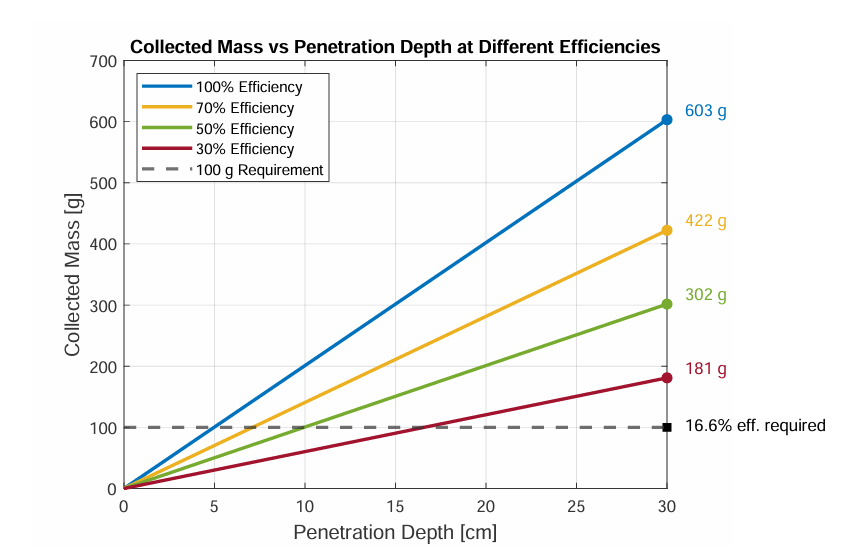
\includegraphics[width=0.70\linewidth]{mass_vs_efficiency.png}
    \caption{Collected mass versus penetration depth for different capture efficiencies.
    The red dashed line indicates the 100~g minimum requirement.}
    \label{fig:mass_efficiency}
\end{figure}




\begin{figure*}
    \centering
    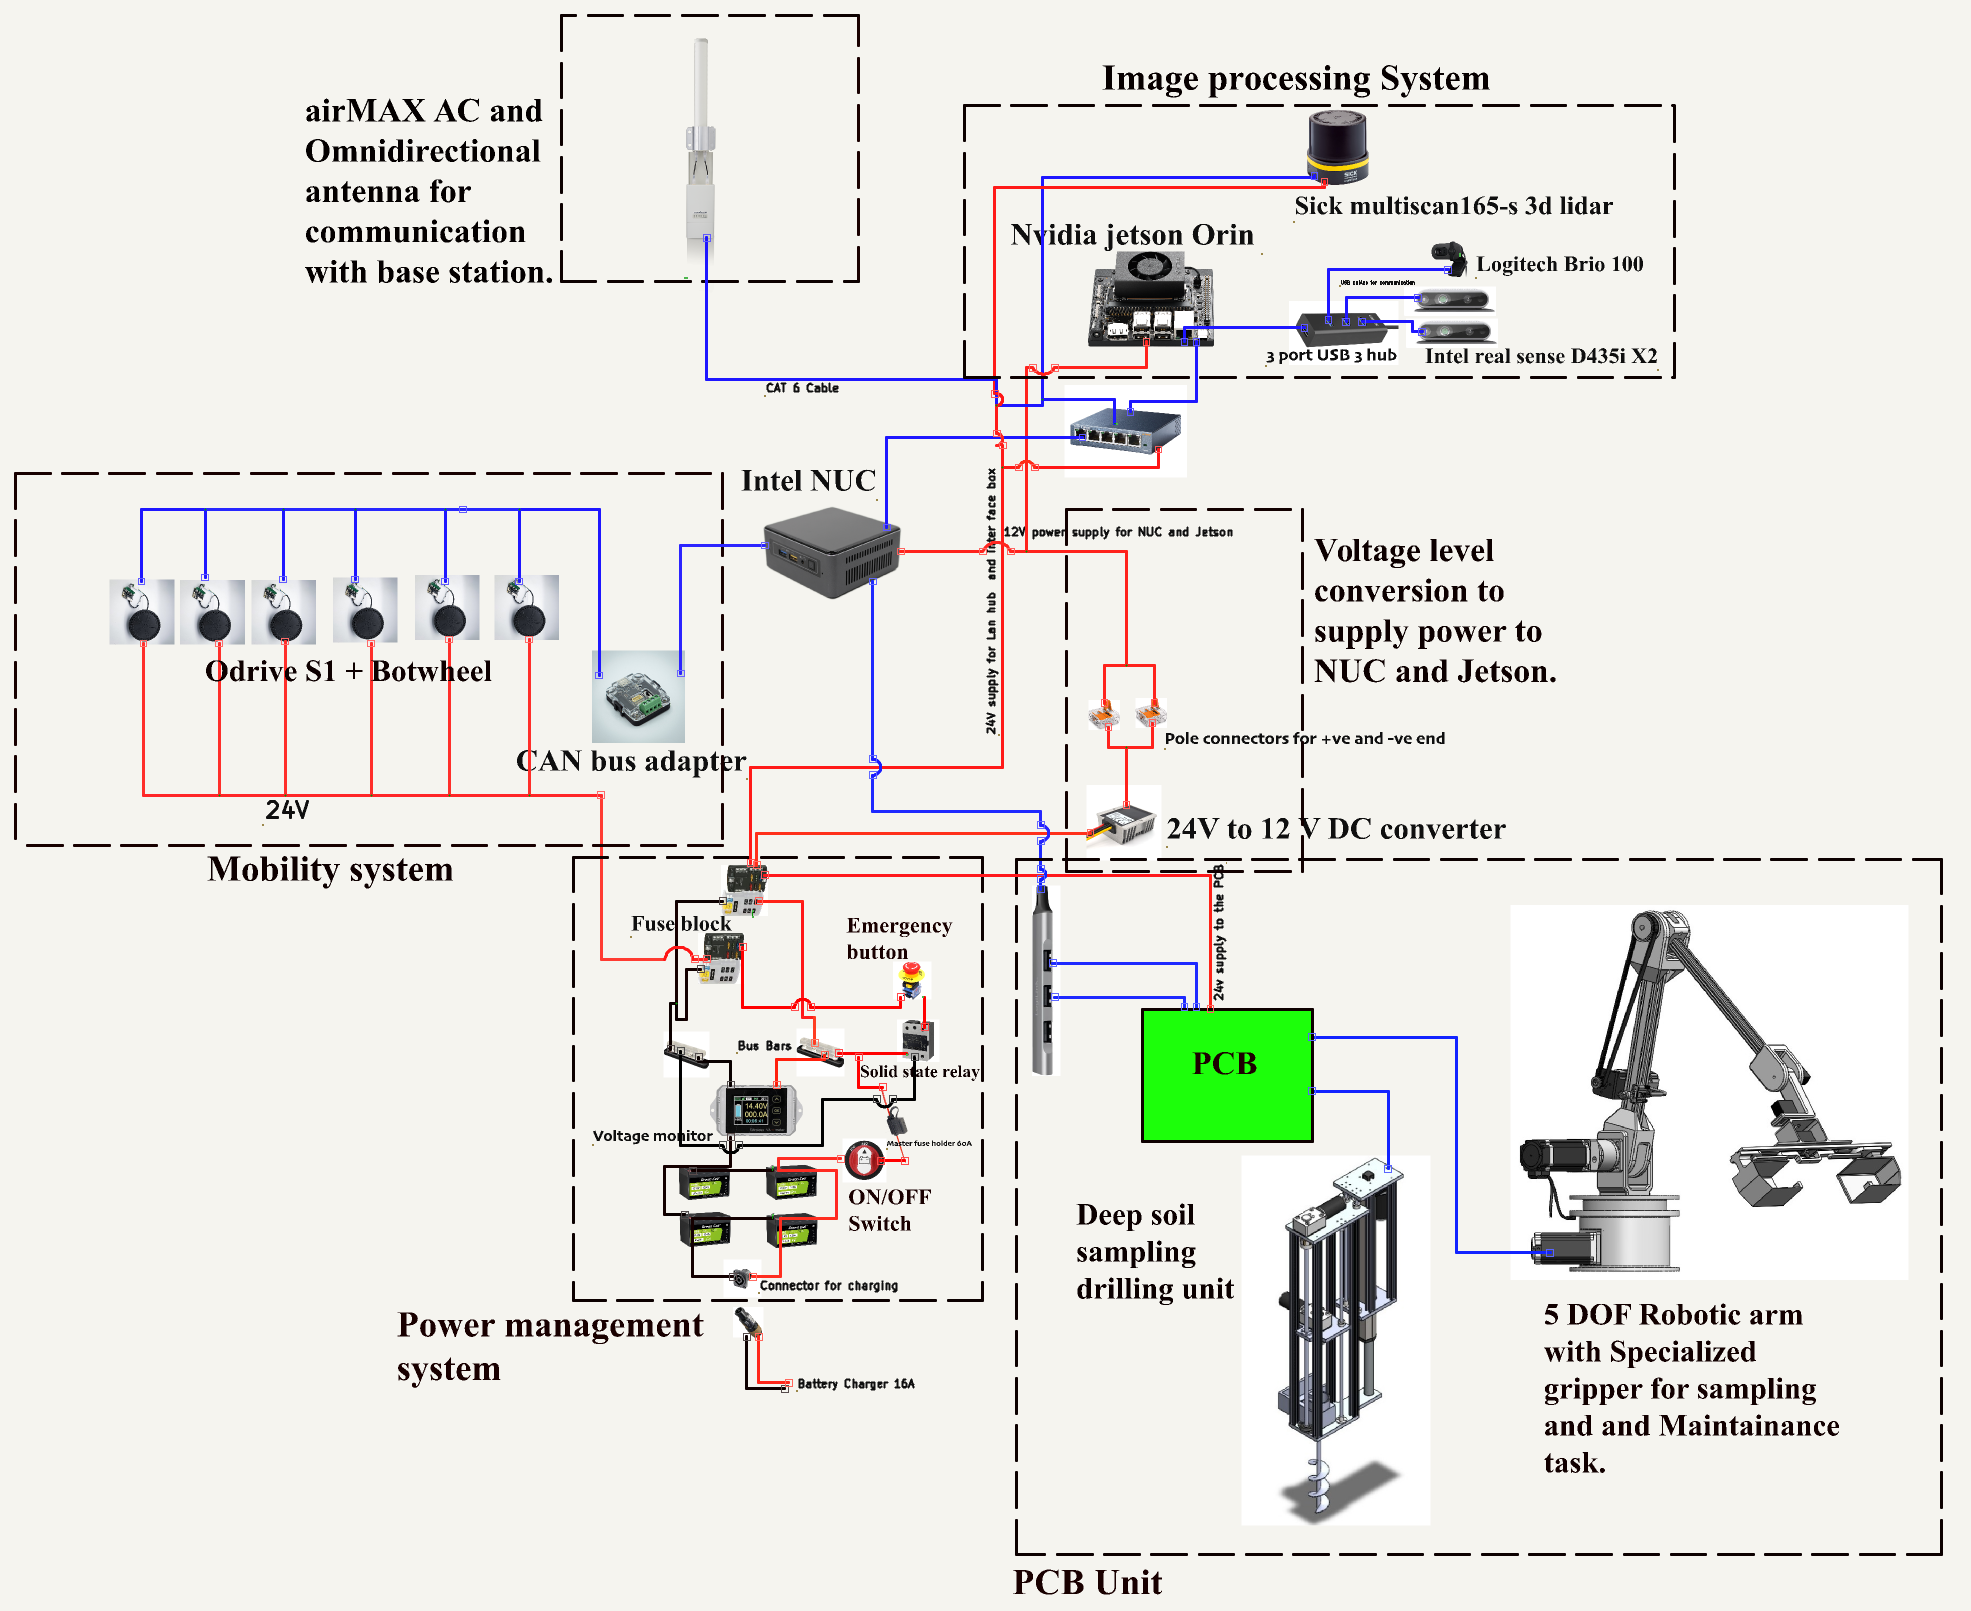
\includegraphics[width=0.7\textwidth]{Elexarch.png}
    \caption{Electrical Architecture}
    \label{elex}
\end{figure*}

\section{ELECTRICAL DESIGN}
This section details the electrical architecture and system design for a six-wheeled autonomous rover developed for the ERC. The design prioritizes robustness, modularity, and operational endurance, critical for navigating challenging Martian terrains. The architecture is built around a centralized 24V LiFePO4 power source, with a dual-voltage power distribution scheme to efficiently supply high-power motor drivers and sensitive, low-voltage computational hardware. A distributed computing model, leveraging an Intel NUC for high and low level control and an NVIDIA Jetson Orin for perception, ensures optimal performance. Furthermore, a custom-designed PCB featuring dual Teensy 4.1 microcontrollers is employed which provides dedicated, real-time control for the robotic arm and drill operations. The following subsections present a comprehensive power budget analysis, battery endurance calculations, and a discussion of key design choices, including safety mechanisms, and power-to-weight considerations. The resulting design is a resilient and high-performance electrical system capable of supporting extended autonomous operations.




\subsection{Power Management System}
The power management system illustrated in Fig. \ref{elex} forms the foundation of the rover’s electrical architecture. It begins with a 24 V, 60 Ah LiFePO4 battery pack, configured in a 2S2P topology from four 12 V, 30 Ah modules. This configuration was chosen to combine the advantages of higher bus voltage, reduced current draw, minimized resistive losses and improved efficiency with the redundancy and load-sharing benefits of parallel operation. The pack provides a total nominal energy of 1.44 kWh, of which up to 98\% is usable, offering sufficient endurance for extended tasks. From the battery, a master fuse rated at 60 A provides pack-level protection against catastrophic faults, while a solid-state relay (SSR) enables controlled connection and disconnection of the traction fuse block. A top-mounted emergency push button directly controls the SSR, allowing immediate isolation of the traction subsystem during unsafe conditions. A keyed master switch is provided for normal on/off operation, ensuring controlled startup and shutdown without relying on the emergency circuit.
The bus bar serves as the central distribution node for the 24 V rail. Branch connections are fused individually, powering the traction system, computational hardware, perception devices, robotic arm and drilling unit. Additional safety and monitoring elements include a battery capacity meter, a charging connector, and a 24 V charger interface, which allow safe recharging without disassembly. This hierarchical distribution strategy localizes faults and simplifies maintenance while providing clean and reliable power to all downstream systems.



\subsection{Mobility System}
The motion control system illustrated in Fig. \ref{elex} provides mobility through six ODrive S1 motor drivers, each paired with a hub-mounted botwheel in the rocker-bogie suspension. The ODrives are supplied directly from the 24 V bus through a fuse block, with individual fuses sized to protect each motor branch. This ensures that a failure in one motor or controller does not compromise the remainder of the traction system. Control communication is achieved through a CAN bus network that daisy-chains all six ODrives. A USB-to-CAN adapter connects the ODrive network to the Intel NUC, enabling higher-level navigation and autonomy software to command the traction system. For redundancy and debugging, direct USB connections to each ODrive are also available. The ODrive S1 supports regenerative braking, and advanced current limiting. With each botwheel rated for 5 A continuous and 15 A peak, the system has ample headroom to deliver the torque required to maneuver the rover across uneven terrain while keeping nominal cruise currents within safe operating margins.

\subsection{Computing System}
The computing system comprises two primary processing units: an Intel NUC and an NVIDIA Jetson Orin NX illustrated in Fig. \ref{elex}. Together, they implement a distributed computing model that separates high-level mission logic from GPU-accelerated perception tasks. The Intel NUC serves as the central mission computer, responsible for high-level navigation, path planning, and coordination between subsystems. It also hosts communications with the base station via the AirMax router and manages CAN bus with the ODrive motor controllers. The NVIDIA Jetson Orin NX provides dedicated GPU resources for real-time perception and autonomy, executing computationally intensive tasks such as visual odometry, SLAM (simultaneous localization and mapping), and object recognition. The Jetson is connected to the perception suite through a powered USB hub, consolidating both data and power delivery.
Both the NUC and Jetson are powered by regulated 12 V rails derived from the 24 V bus through high-efficiency DC-DC converters. Each converter feed is individually fused to prevent cascading faults and to ensure stable voltage delivery under transient load conditions. Centralizing the conversion stages in a single block reduces thermal stress, simplifies filtering, and enables enable-pin control tied into the emergency stop logic.

\subsection{Sensor System}
The sensor system enables the rover’s autonomous perception and teleoperation capabilities. It integrates a Sick MultiScan 3D LiDAR, two Intel RealSense D435i depth cameras, and a Logitech Brio webcam as shown in Fig. \ref{elex}. The Sick LiDAR, powered directly from the 24 V rail, provides 3D mapping data for navigation and obstacle detection. The Intel RealSense cameras, powered via 5 V from the USB hub, deliver stereo depth perception that supports close-range hazard detection and manipulation tasks. The Logitech Brio webcam supplements this suite during drilling and sampling operations, offering a wide-field visual feed for teleoperation and surface/deep sample verification. These devices collectively draw approximately 34 W and are routed through a powered USB 3 hub connected to the Jetson Orin NX. Consolidating data through a single hub reduces cabling complexity and allows unified bandwidth management. Mounting the sensors on the rover mast reduces occlusion by the chassis and ensures optimal visibility for both autonomy and remote operation. Each perception device is protected by dedicated fusing, ensuring that a single sensor fault does not disable the entire vision system.

\subsection{Printed Circuit Board}
To coordinate the complex operations of the robotic arm and deep soil drill, the rover employs a custom-designed Printed Circuit Board (PCB), which acts as a dedicated control hub. This PCB offloads real-time control tasks from the Intel NUC and Jetson, ensuring that high-frequency actuator commands and sensor readings do not interfere with higher-level computation.
The board is designed around two Teensy 4.1 microcontrollers, configured as slaves to the Intel NUC. They are selected for their high clock speeds (600 MHz), low-latency I/O handling, and flexibility in real-time embedded applications. Responsibilities are divided between the two controllers:
\begin{itemize}
    \item Teensy A manages the robotic arm’s kinematics, controlling five degrees of freedom via two CL57T and one CL42T stepper motor drivers, in addition to three Muizei 25 kg servo motors. This enables precise positioning and manipulation during sample collection and maintenance tasks.
    \item Teensy B governs the deep soil drill module, handling drill deployment, actuation, and concurrent data acquisition from auxiliary sensors such as an Inertial Measurement Unit (IMU) for orientation feedback.
\end{itemize}

Since the Teensy microcontrollers operate at a 3.3 V logic level, the PCB integrates bi-directional logic-level shifters to interface safely with external 5 V motor drivers and peripherals. Additionally, onboard voltage regulators step down the 24 V supply to stable 5 V and 3.3 V rails dedicated to the control electronics, isolated from noise-prone motor circuits. This dual-MCU architecture improves modularity and resilience: the robotic arm and drill can operate independently, and a failure in one control loop does not propagate to the other. Furthermore, the PCB incorporates diagnostic interfaces and communication ports that allow status monitoring and debugging during ERC field operations. By offloading actuator-intensive tasks to the PCB, the system ensures that the main computers (NUC and Jetson) can prioritize autonomy, navigation, and perception tasks without being bottlenecked by low-level actuator control. This enhances determinism, system reliability, and mission capability, aligning with the modular and fault-tolerant philosophy of the overall electrical design.


\section{COMMUNICATION DESIGN}
The communication system for the rover is explained in this section. As per the ERC rule book, the rover’s radio communication shall comply with legally available frequencies and power levels, with a maximum distance between the rover and antenna mast of 100 meters. Line-of-sight between control base and rover antennas may be occluded by terrain. Standard 2.4 GHz Wi-Fi (2412–2472 MHz, IEEE 802.11 b/g/n, max 100mW EIRP) is accepted, with only one 20MHz channel per rover. The 5 GHz low band (5150–5725MHz) allows two 80MHz channels for Wi-Fi and AirMax, up to 1W EIRP. The 5 GHz high band (5725–5875MHz) allows two 30 MHz channels. ISM bands may be used within European regulations, with documented compliance.


\subsection{Communication Architecture}
\begin{figure}[htbp]
    \centering
    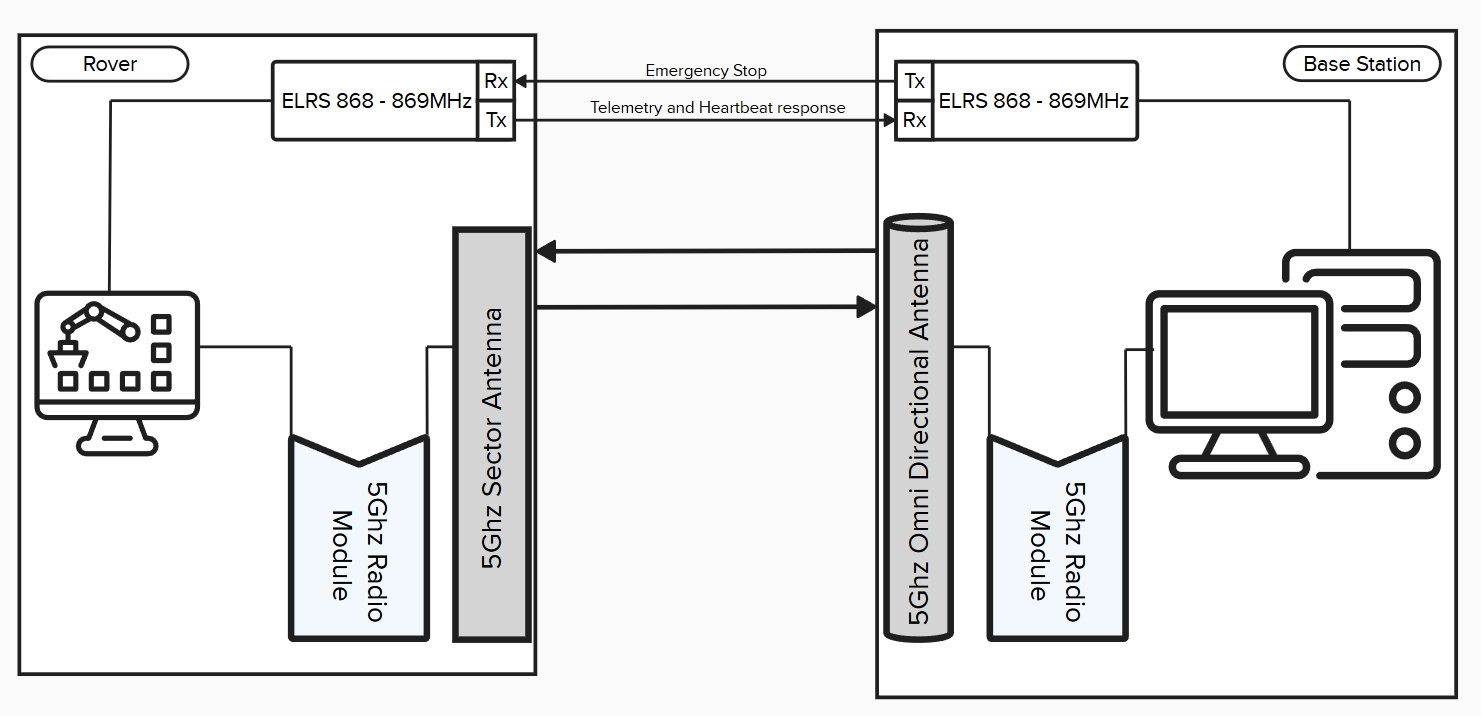
\includegraphics[width=1\linewidth]{figures/Communication_setup.png}
    \caption{Communication Architecture of HSM Aries Leap One}
    \label{fig:placeholder}
\end{figure}
The primary communication challenges for the rover include latency, terrain occlusions, interference, and EIRP restrictions. The base station uses a high-gain sector antenna (18.6–19.1dBi) with a wide horizontal beamwidth of 123° and a slight electrical downtilt, ensuring focused coverage over the rover’s operational area. The rover employs a 10dBi omnidirectional antenna with a 12° vertical beamwidth to maintain connectivity during rotation or changes in orientation. Both antennas feature dual-linear polarization and good cross-polar isolation, which reduces interference and improves link quality. For robust low-latency telemetry, heartbeat monitoring, and emergency stop functionality, ELRS modules operating at 868–869 MHz are employed alongside the existing network infrastructure. The base station ELRS transmitter sends heartbeat signals and emergency stop commands to the rover, while the ELRS receiver on the rover captures these instructions in real time. Telemetry from the rover, including sensor readings and status information, is transmitted back to the base station via the ELRS link. The ELRS modules interface with the base station and rover controllers using UART-to-USB converters, enabling connection to a computer for monitoring, logging, and control. This configuration ensures ultra-low latency for emergency stop signals, maintaining reliable operation even in environments with high interference or partial terrain occlusions. 
\begin{table}[h!]
\centering
\caption{Specifications of the airMAX Rocket AC Lite radio module}
\begin{tabular}{|l|l|}
\hline
\textbf{Parameter} & \textbf{Value} \\ \hline
Networking Interface & 1 × GbE RJ45 port \\ \hline
Power Method & Passive PoE 24V (2-pair) \\ \hline
Max. Power Consumption & 8.5 W \\ \hline
Management Radio (MHz) & 5150–5875 MHz \\ \hline
\end{tabular}
\end{table}

The 5GHz radio modules operate over 5.15–5.875 GHz for standard IP networking, powered via Passive PoE 24V (2-pair) with 8.5W consumption. Networking is handled over standard IP, with UDP for high-bandwidth telemetry data and TCP for control commands, ensuring low latency and reliable command delivery.



\begin{table}[h!]
\centering
\caption{Specifications of airMAX Sector and Omni-Directional Antennas}
\begin{tabular}{|l|c|c|}
\hline
\textbf{Parameter} & \textbf{Sector} & \textbf{Omni-Directional} \\ \hline
Frequency Range & 5.15 – 5.85 GHz & 5.45 – 5.85 GHz \\ \hline
Gain & 18.6 – 19.1 dBi & 10 dBi \\ \hline
Beamwidth & 123° & 360° \\ \hline
Electrical Beamwidth & 4° & 12° \\ \hline
Electrical Downtilt & 2° & 4° \\ \hline
Polarization & Dual-Linear & Dual-Linear \\ \hline
Cross-Polar Isolation & ≥ 28 dB & ≥ 25 dB \\ \hline
Max. VSWR & 1.5:1 & 1.6:1 \\ \hline
\end{tabular}
\end{table}


\begin{figure}[htbp]
    \centering
    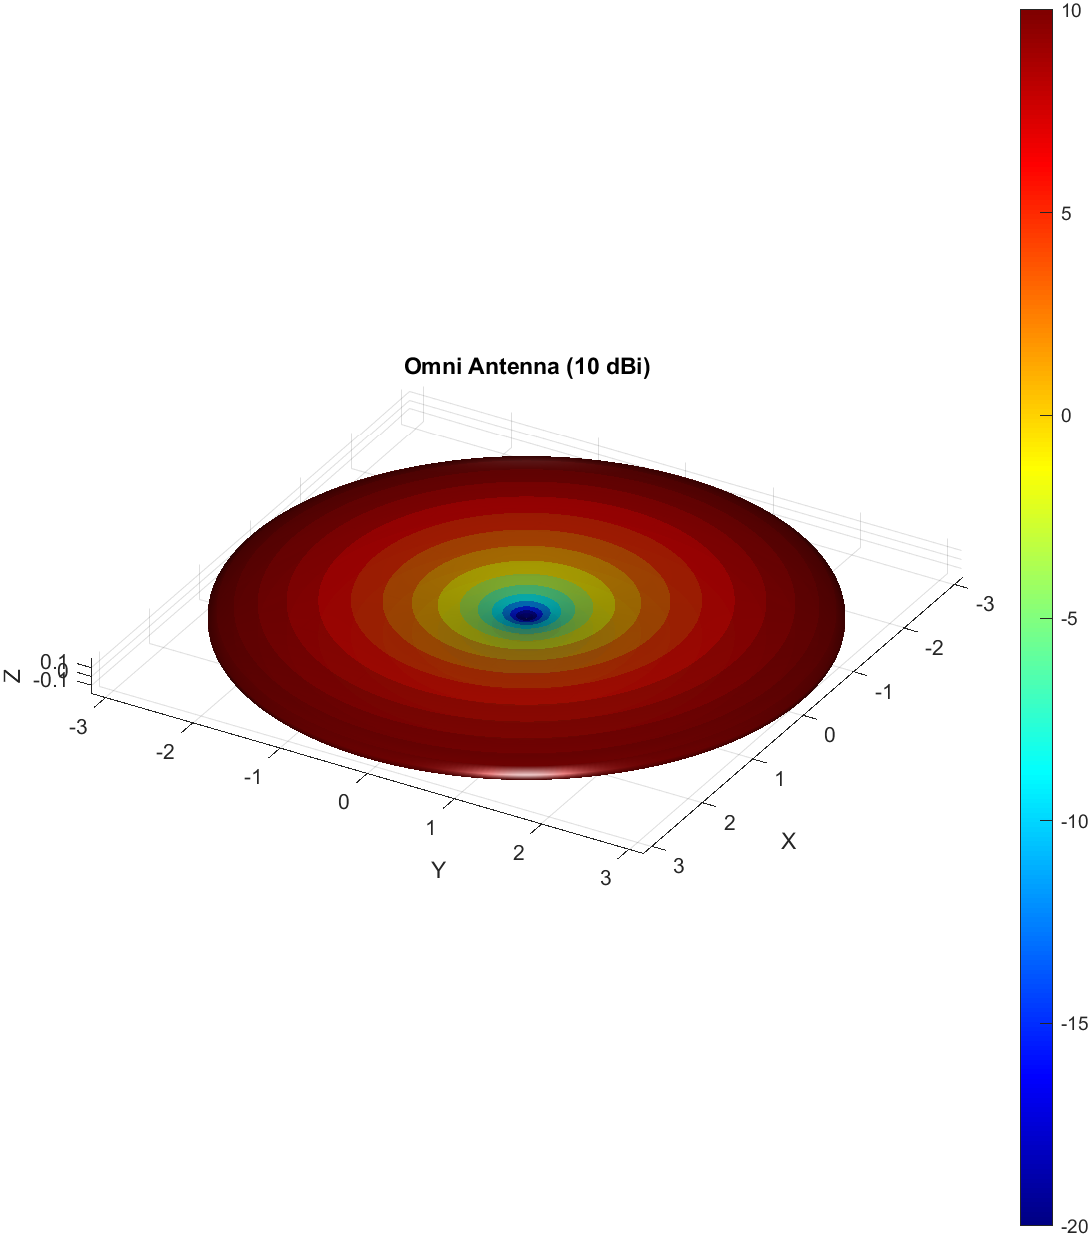
\includegraphics[width=0.7\linewidth]{figures/omni.png}
    \caption{Omni Directional Antenna Radiation Pattern. Gain distribution is shown in azimuth and elevation planes.}
    \label{fig:placeholder}
\end{figure}

\subsection{Calculations:}
In this section, the key parameters of the rover communication link are calculated to evaluate its performance. The Free Space Path Loss (FSPL) is determined based on the operating frequency and distance, providing an estimate of signal attenuation over the link. Using FSPL, transmit power, antenna gains, and cable losses, the received power of the rover is computed. The receiver noise figure (NF) and the system bandwidth are then used to estimate the noise floor, which, combined with the received power, allows calculation of the signal-to-noise ratio (SNR). Finally, the link margin is obtained by comparing the received power to the minimum receiver sensitivity, indicating the robustness of the communication link under the given operating conditions. These calculations demonstrate that the selected hardware ensures reliable telemetry and control within the expected operational range.

\subsubsection*{System Parameters}

The assumed system parameters are as follows:

\begin{itemize}
    \item Frequency: $f = 5.8 \,\text{GHz}$ (mid-point of the high band).
    \item Distance: $d = 100 \,\text{m}$.
    \item Transmit power: $P_t = 22 \,\text{dBm}$ (average, 22–27 dBm for R5AC-Lite).
    \item Maximum EIRP: $\leq 30 \,\text{dBm}$ (regulatory limit).
    \item Transmitter path loss: $L_{\text{TX}} = 2 \,\text{dB}$.
    \item Transmitter antenna gain: $G_t = 10 \,\text{dBi}$.
    \item Receiver antenna gain: $G_r = 19.1 \,\text{dBi}$.
    \item Receiver sensitivity: $-65 \pm 2 \,\text{dBm}$ (for $8 \times 256$ QAM, 5/6 coding).
    \item Channel bandwidth: $B = 30 \,\text{MHz}$.
    \item Receiver noise figure: $NF = 6 \,\text{dB}$.
    \item Cable losses: $L_c = 2 \,\text{dB}$.
\end{itemize}

The Effective Isotropic Radiated Power (EIRP) is given by:
\begin{equation}
    \mathrm{EIRP} = P_t - L_{\mathrm{TX}} - L_c + G_t,
\end{equation}


\subsubsection{Calculation of Free Space Path Loss}
\begin{align*}
\text{FSPL (dB)} &= 20 \log_{10}(d) + 20 \log_{10}(f) + 32.44 \\
\text{FSPL} &= 20 \log_{10}(0.1) + 20 \log_{10}(5800) + 32.44 \\= \textbf{75.26 \text{ dB}} \\
\end{align*}

\subsubsection{Calculation of Receiver Power}
\begin{align*}
P_r &= P_t + G_t + G_r - \text{FSPL} - L \\
\text{FSPL} &= 87.7\ \text{dB} \\
P_r &\approx -38.6\ \text{dBm}
\end{align*}
\subsubsection{Noise Floor Calculation}
\begin{align*}
B &= 30\ \text{MHz} = 3 \times 10^7\ \text{Hz} \\
10 \log_{10}(B) &= 10 \log_{10}(3 \times 10^7) \\
= 74.77\ \text{dB} \\
NF &= 6\ \text{dB (typical)} \\
N &= -174 + 10 \log_{10}(B) + NF \\
&\approx -93.23\ \text{dBm}
\end{align*}

\subsubsection{Signal-to-Noise Ratio (SNR) Calculation}
\begin{align*}
SNR &= P_r - N \\
&\approx 54.63\ \text{dB}
\end{align*}

\subsubsection{Link Margin Calculation}
\begin{align*}
P_{\min} &= -65\ \text{dBm (required for stable Wi-Fi)} \\
\text{Link Margin} &= P_r - P_{\min} \\
&\approx 26.4\ \text{dB}
\end{align*}

\begin{figure}[htbp]
    \centering
    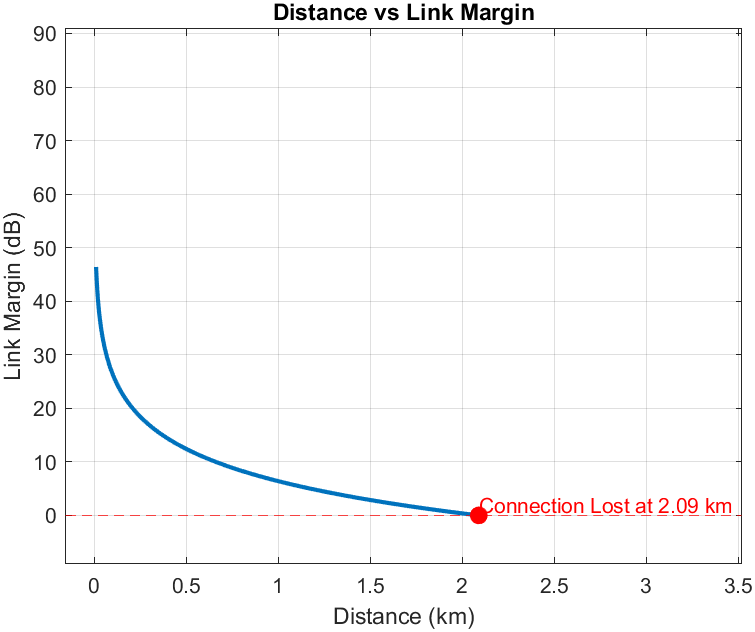
\includegraphics[width=0.75\linewidth]{figures/lm.png}
    \caption{Distance vs Link Margin}
    \label{fig:placeholder}
\end{figure}

\subsection{Validation of Objective}



The calculations above summarize the key parameters of the link budget for the 0.1~km 5.8~GHz link. FSPL of 87.7 dB represents the free-space attenuation. The calculated received power of -38.6 dBm is well above the receiver sensitivity (-65 dBm ± 2 dB), providing a high SNR of 54.63 dB. The resulting link margin of 26.4 dB indicates a very robust link, ensuring reliable communication even with additional environmental losses.

\begin{figure}[htbp]
    \centering
    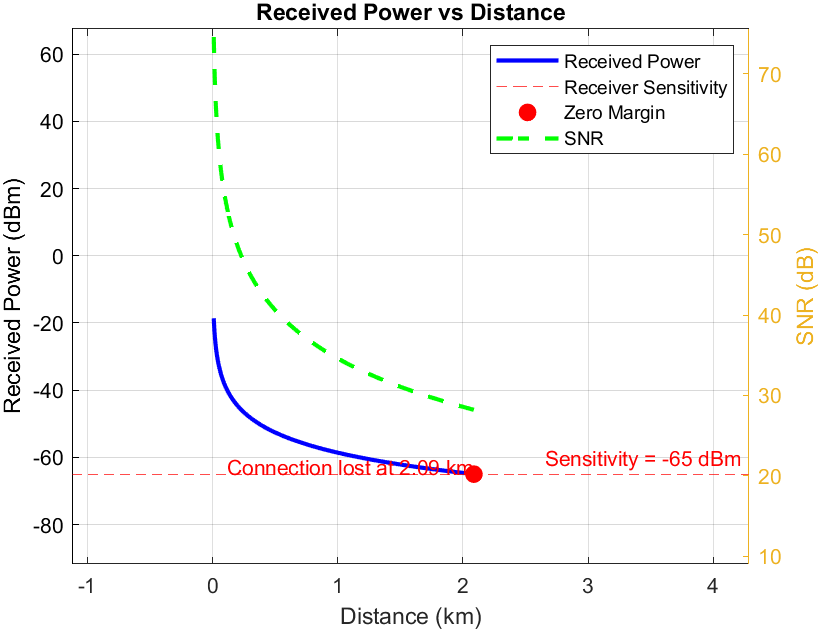
\includegraphics[width=0.75\linewidth]{figures/snr.png}
    \caption{Received Power and SNR vs Distance}
    \label{fig:placeholder}
\end{figure}

Assuming perfect antenna alignment and free-space conditions with no obstacles, the calculated maximum link distance is $2.09 \,\text{km}$. However, in practice, the achievable range will always be lower due to 
environmental factors such as multipath fading, atmospheric absorption, 
antenna misalignment, and unforeseen obstructions. 


\section{CONCLUSION}

\section{FUTURE SCOPE}


\addtolength{\textheight}{-12cm}   % Balance the last page columns

%%%%%%%%%%%%%%%%%%%%%%%%%%%%%%%%%%%%%%%%%%%%%%%%%%%%%%%%%%%%%%%%%%%%%%%%%%%%%%%%





\begin{thebibliography}{99}
\bibitem{marstestbed} M. Azkarate, L. Gerdes, T. Wiese, M. Zwick, M. Pagnamenta, J. Hidalgo-Carrió, P. Poulakis, and C. J. Pérez-del Pulgar, "Design, Testing, and Evolution of Mars Rover Testbeds," IEEE Robotics \& Automation Magazine, vol. 29, no. 3, pp. 10–25, Sept. 2022, doi: 10.1109/MRA.2021.3134875.
\bibitem{mobsub} R. Lindemann, et al., “Mobility Sub-System for the Exploration Technology Rover,” Proc. Of the 33rd Aerospace Mechanisms Symposium, Pasadena CA,
NASA/CP-1999-209259, pp. 115-130, 19-21 May 1999.
\bibitem{sherpasus}Cordes, Florian \& Kuehn, Daniel \& Oekermann, Christian \& Babu, Ajish \& Stark, Tobias \& Kirchner, Frank. (2014). An Active Suspension System for a Planetary Rover. 

\bibitem{ERC20} A. Losiak et al., "Mars Yard Design During the European Rover Challenge (ERC) 2020-2022," in Proc. 54th Lunar and Planetary Science Conference, vol. 2806, 2023.


\bibitem{aries}HSMaries Mars Rover Team. “HS Maries Space,” Accessed: Aug. 18, 2025. [Online]. Available: https://hsmaries.space/
\bibitem{b1}Lindemann, R.A. ; Voorhees, C.J.: Mars Exploration Rover mobility assembly design, test and performance. In: Systems, Man and Cybernetics, 2005, IEEE International Conference on Bd. 1, 2005, pp. 450--455, vol. 1
\bibitem{b2} Mishkin, A.H. ; Morrison, J.C. ; Nguyen, T.T. ; Stone, H.W. ; Cooper, B.K. ; Wilcox, B.H.: Experiences with operations and autonomy of the Mars Pathfinder Microrover. In: Aerospace Conference, 1998.

\bibitem{b3} NASA JPL. Homepage of Curiosity Mission. Web. April 2014

\bibitem{b4} D. Bickler, “Roving over Mars,” Mechanical
Engineering Magazine, American Society of Mechanical
Engineers, April 1998.

\bibitem{b5} Vandi Verma et al., Autonomous robotics is driving Perseverance rover’s progress on Mars.Sci.Robot.8,eadi3099(2023).DOI:10.1126/scirobotics.adi3099

\bibitem{b6} C. R. Weisbin, G. Rodriguez, P. S. Schenker, H. Das, S. A. Hayati, E. T. Baumgartner, M. Maimone, I. A. Nesnas, and R. A. Volpe, "Autonomous Rover Technology for Mars Sample Return," presented at the IEEE Aerospace Conference, Big Sky, MT, USA, Mar. 1999. [Online]. Available: \url{https://www.ri.cmu.edu/pub_files/pub2/weisbin_c_1999_1/weisbin_c_1999_1.pdf}


\bibitem{b7}Hayati, R. Volpe, P. Backes, J. Balaram, R. Welch, R. Ivlev, G. Tharp, S. Peters, T. Ohm, R. Petras, S. Laubach, “The Rocky 7 rover: a Mars sciencecraft prototype” Proc. International Conference on Robotics and Automation, 1997. Volume: 3 , Page(s): 2458 –2464

\bibitem{harrington2004}
B.~D. Harrington and C.~J. Voorhees,
``The Challenges of Designing the Rocker--Bogie Suspension for the Mars Exploration Rover,''
\emph{Proc. 37th Aerospace Mechanisms Symposium}, NASA, 2004.
Available: \url{https://ntrs.nasa.gov/citations/20040084284}.

\bibitem{rivellini1993}
T.~P. Rivellini,
``Mechanisms of the Rocky IV Rover,''
\emph{Proc. 27th Aerospace Mechanisms Symposium}, 1993, pp. 19--34.
Available: \url{https://ntrs.nasa.gov/api/citations/19940025127/downloads/19940025127.pdf}.


\bibitem{papadopoulos1996}
E.G. Papadopoulos and D.A. Rey,
`A New Measure of Tipover Stability Margin for Mobile Manipulators,'
in \emph{Proc. IEEE International Conference on Robotics and Automation (ICRA)}, 1996, pp. 3111--3116.
doi: 10.1109/ROBOT.1996.509193.

\bibitem{kelly2005}
A.~Kelly and A.~Diaz-Calderon,
``On-Line Stability Margin and Attitude Estimation for Dynamic Articulating Mobile Robots,''
\emph{International Journal of Robotics Research}, vol.~24, no.~10, pp.~845--866, 2005.
doi: 10.1177/0278364905057059.

\bibitem{tk5754}
thyssenkrupp Materials,
``EN AW-5754 (AlMg3) Aluminium Alloy -- Data Sheet,'' 2018.
Available: \url{https://www.thyssenkrupp-materials.co.uk/media/20051/en-aw-5754.pdf}.

\bibitem{rb5754h111}
Righton Blackburns,
``Aluminium Alloy 5754 H111 -- Sheet \& Plate (BS EN 485-2),'' 2024.
Available: \url{https://www.rightonblackburns.co.uk/datasheets/view/Righton-Blackburns-Ltd_Aluminium-Alloy-5754-H111-Sheet-Plate_142.pdf}.

\bibitem{tk5754h22}
thyssenkrupp Materials,
``Aluminium Alloy 5754 H22/H24/H26 -- Data Sheet,'' 2016.
Available: \url{https://www.thyssenkrupp-materials.co.uk/media/19614/en-aw-5754-h22_h24_h26.pdf}.

\bibitem{ERC} European Rover Challenge, "ERC-2025-RULES-Rev.3.1.pdf," July 8, 2025. [Online]. Available: \url{https://drive.google.com/drive/folders/1KdcoDvAagL5XTdI4Df0xQ4lTry5U_2Hv}. Accessed: Aug. 18, 2025.

\bibitem{odriveBotwheelDocs}
ODrive Robotics, ``ODrive Motors — ODrive BotWheel,'' Documentation (vLatest), accessed: Aug. 18, 2025. [Online]. Available:
\url{https://docs.odriverobotics.com/v/latest/hardware/odrive-motors.html#odrive-botwheel}.

\bibitem{odriveBotwheelsShop}
ODrive Robotics, ``ODrive BotWheels — Specifications,'' accessed: Aug. 18, 2025. [Online]. Available:
\url{https://shop.odriverobotics.com/products/odrive-botwheels}.

\end{thebibliography}

\end{document}
